\section{Results}
\label{sec:3-results}
The results section will: 1. introduce the data instance from the case company;
2. show the effect of forcing work orders into specific weekly schedules $
\ElementPeriod \in \SetPeriod$; 3. show the effect of changing the  period
capacities $\ParStrategicResource$, and 4. show the effect of dynamically
changing the $\ParStrategicValue$ associated with $\ElementPeriod \in
\SetPeriod$ and $\ElementWorkOrder \in \SetWorkOrder$.
\definecolor{red}{HTML}{8A3F3A}
\definecolor{yellow}{HTML}{E0BB3C}
\definecolor{blue}{HTML}{4569E0}
\definecolor{green}{HTML}{17E561}
\definecolor{other}{HTML}{6A939E}

% DTU Colors
\definecolor{dtu-corporate-red}{HTML}{990000}
\definecolor{dtu-white}{HTML}{ffffff}
\definecolor{dtu-black}{HTML}{000000}
\definecolor{dtu-blue}{HTML}{2F3EEA}
\definecolor{dtu-bright-green}{HTML}{1FD082}
\definecolor{dtu-navy-blue}{HTML}{030F4F}
\definecolor{dtu-yellow}{HTML}{F6D04D}
\definecolor{dtu-orange}{HTML}{FC7634}
\definecolor{dtu-pink}{HTML}{F7BBB1}
\definecolor{dtu-grey}{HTML}{DADADA}
\definecolor{dtu-red}{HTML}{E83F48}
\definecolor{dtu-green}{HTML}{008835}
\definecolor{dtu-purple}{HTML}{79238E}

\subsection{Data Instance}
\begin{table}[H]
\centering
\begin{tabular}{|c|c|c|c|c|}
\hline
           & \begin{tabular}[c]{@{}c@{}}$|\SetWorkOrder{}|$\end{tabular} & \begin{tabular}[c]{@{}c@{}}$|\SetResource|$\end{tabular} & \begin{tabular}[c]{@{}c@{}}$|\SetPeriod|$\end{tabular} \\ \hline
Instance 1 & 3487                                                          & 16                                                               & 52                                                            \\ \hline
\end{tabular}

\caption{List of data instances from the case company. Here $\SetWorkOrder$ is the set of work orders, $\SetResource$ is the set of resources, and $\SetPeriod$ is the set of weekly periods.} % \label{fig1}
\end{table}

\subsection{Response to Inclusion}
The response to the inclusion of a work order is given by I parameter of the model which 
is constrained in \ref{eqn:constraint:strategic:include} of model given in .

The inclusion is made of forcing certain allocations of work orders to be in specific periods. Below a table is provided 
to show what changes will occur and at what and at what point in time.
\begin{table}[H]
	\centering
	\begin{tabular}{|c|c|c|c|c|c|}
	\hline
	\begin{tabular}[c]{@{}c@{}}\end{tabular}     & \begin{tabular}[c]{@{}c@{}}$\VarMetaTime_1 = 60$\end{tabular} & \begin{tabular}[c]{@{}c@{}} $\VarMetaTime_2 = 120$ \end{tabular} & \begin{tabular}[c]{@{}c@{}}$\VarMetaTime_3 = 180$\end{tabular} & \begin{tabular}[c]{@{}c@{}}$\VarMetaTime_4 = 240$\end{tabular} & \begin{tabular}[c]{@{}c@{}}$\VarMetaTime_5 = 300$\end{tabular} \\ \hline
	\begin{tabular}[c]{@{}c@{}}$\Delta |\SetPeriod|$\end{tabular} & 10                                                       & 20                                                       & 30                                                       & 40                                                       & 50                                                       \\ \hline
	\end{tabular}
\end{table}

With the inputs defined we will explain the main results which are shown in the figure below. 
\begin{figure}[H]
	\centering
	\pgfplotsset{compat=1.18}
	\pgfplotsset{
	    every axis/.append style={
	        font=\small, % Use document font size
	        axis line style={dtu-red}, % Axis lines
	        tick label style={dtu-green}, % Tick labels
	        label style={myblue}, % Axis labels
	        title style={myred} % Title in custom red
	    },
	    grid style={dashed,gray}, % Customize gridlines
	    every axis plot/.append style={very thick} % Thick lines
	}
	\resizebox{\linewidth}{!}{
		\tikzpicture[gnuplot]
%% generated with GNUPLOT 6.0p1 (Lua 5.2; terminal rev. Jun 2020, script rev. 118)
%% Mon 02 Dec 2024 07:56:47 PM UTC
\path (0.000,0.000) rectangle (16.000,12.000);
\gpcolor{color=gp lt color border}
\gpsetlinetype{gp lt border}
\gpsetdashtype{gp dt solid}
\gpsetlinewidth{1.00}
\draw[gp path] (2.424,2.881)--(2.604,2.881);
\draw[gp path] (15.447,2.881)--(15.267,2.881);
\node[gp node right] at (2.240,2.881) {$1.9\times10^{11}$};
\draw[gp path] (2.424,4.052)--(2.604,4.052);
\draw[gp path] (15.447,4.052)--(15.267,4.052);
\node[gp node right] at (2.240,4.052) {$1.91\times10^{11}$};
\draw[gp path] (2.424,5.222)--(2.604,5.222);
\draw[gp path] (15.447,5.222)--(15.267,5.222);
\node[gp node right] at (2.240,5.222) {$1.92\times10^{11}$};
\draw[gp path] (2.424,6.393)--(2.604,6.393);
\draw[gp path] (15.447,6.393)--(15.267,6.393);
\node[gp node right] at (2.240,6.393) {$1.93\times10^{11}$};
\draw[gp path] (2.424,7.563)--(2.604,7.563);
\draw[gp path] (15.447,7.563)--(15.267,7.563);
\node[gp node right] at (2.240,7.563) {$1.94\times10^{11}$};
\draw[gp path] (2.424,8.734)--(2.604,8.734);
\draw[gp path] (15.447,8.734)--(15.267,8.734);
\node[gp node right] at (2.240,8.734) {$1.95\times10^{11}$};
\draw[gp path] (2.424,9.904)--(2.604,9.904);
\draw[gp path] (15.447,9.904)--(15.267,9.904);
\node[gp node right] at (2.240,9.904) {$1.96\times10^{11}$};
\draw[gp path] (2.424,11.075)--(2.604,11.075);
\draw[gp path] (15.447,11.075)--(15.267,11.075);
\node[gp node right] at (2.240,11.075) {$1.97\times10^{11}$};
\draw[gp path] (2.424,2.881)--(2.424,2.701);
\draw[gp path] (2.424,11.075)--(2.424,11.255);
\node[gp node left,rotate=270] at (2.424,2.517) {$1.73317\times10^{9}$};
\draw[gp path] (4.052,2.881)--(4.052,2.701);
\draw[gp path] (4.052,11.075)--(4.052,11.255);
\node[gp node left,rotate=270] at (4.052,2.517) {$1.73317\times10^{9}$};
\draw[gp path] (5.680,2.881)--(5.680,2.701);
\draw[gp path] (5.680,11.075)--(5.680,11.255);
\node[gp node left,rotate=270] at (5.680,2.517) {$1.73317\times10^{9}$};
\draw[gp path] (7.308,2.881)--(7.308,2.701);
\draw[gp path] (7.308,11.075)--(7.308,11.255);
\node[gp node left,rotate=270] at (7.308,2.517) {$1.73317\times10^{9}$};
\draw[gp path] (8.936,2.881)--(8.936,2.701);
\draw[gp path] (8.936,11.075)--(8.936,11.255);
\node[gp node left,rotate=270] at (8.936,2.517) {$1.73317\times10^{9}$};
\draw[gp path] (10.563,2.881)--(10.563,2.701);
\draw[gp path] (10.563,11.075)--(10.563,11.255);
\node[gp node left,rotate=270] at (10.563,2.517) {$1.73317\times10^{9}$};
\draw[gp path] (12.191,2.881)--(12.191,2.701);
\draw[gp path] (12.191,11.075)--(12.191,11.255);
\node[gp node left,rotate=270] at (12.191,2.517) {$1.73317\times10^{9}$};
\draw[gp path] (13.819,2.881)--(13.819,2.701);
\draw[gp path] (13.819,11.075)--(13.819,11.255);
\node[gp node left,rotate=270] at (13.819,2.517) {$1.73317\times10^{9}$};
\draw[gp path] (15.447,2.881)--(15.447,2.701);
\draw[gp path] (15.447,11.075)--(15.447,11.255);
\node[gp node left,rotate=270] at (15.447,2.517) {$1.73317\times10^{9}$};
\draw[gp path] (2.424,11.075)--(2.424,2.881)--(15.447,2.881)--(15.447,11.075)--cycle;
\gpcolor{rgb color={0.580,0.000,0.827}}
\draw[gp path] (3.270,9.933)--(3.270,9.772)--(3.270,9.494)--(3.270,9.436)--(3.303,9.421)%
  --(3.303,9.358)--(3.303,9.291)--(3.303,9.005)--(3.303,8.972)--(3.303,8.930)--(3.303,8.908)%
  --(3.303,8.879)--(3.303,8.773)--(3.336,8.743)--(3.336,8.602)--(3.336,8.511)--(3.336,8.442)%
  --(3.336,8.400)--(3.336,8.296)--(3.336,8.218)--(3.336,8.178)--(3.336,8.145)--(3.368,8.127)%
  --(3.368,8.069)--(3.368,7.994)--(3.368,7.922)--(3.368,7.828)--(3.368,7.811)--(3.401,7.810)%
  --(3.401,7.791)--(3.401,7.776)--(3.401,7.774)--(3.401,7.619)--(3.401,7.590)--(3.401,7.564)%
  --(3.433,7.557)--(3.433,7.530)--(3.433,7.440)--(3.433,7.437)--(3.433,7.434)--(3.433,7.413)%
  --(3.433,7.397)--(3.466,7.370)--(3.466,7.369)--(3.466,7.353)--(3.466,7.264)--(3.466,7.148)%
  --(3.498,7.126)--(3.498,7.121)--(3.498,6.986)--(3.498,6.933)--(3.531,6.788)--(3.531,6.740)%
  --(3.531,6.729)--(3.564,6.727)--(3.564,6.657)--(3.564,6.648)--(3.564,6.591)--(3.596,6.529)%
  --(3.596,6.499)--(3.629,6.489)--(3.629,6.486)--(3.629,6.476)--(3.629,6.444)--(3.629,6.409)%
  --(3.661,6.408)--(3.661,6.407)--(3.661,6.387)--(3.694,6.348)--(3.694,6.335)--(3.726,6.315)%
  --(3.726,6.274)--(3.726,6.221)--(3.759,6.190)--(3.759,6.187)--(3.759,6.168)--(3.759,6.131)%
  --(3.791,6.124)--(3.824,6.077)--(3.824,6.017)--(3.857,6.011)--(3.857,5.993)--(3.857,5.986)%
  --(3.857,5.984)--(3.889,5.938)--(3.889,5.929)--(3.889,5.880)--(3.922,5.871)--(3.922,5.823)%
  --(3.922,5.794)--(3.922,5.758)--(3.954,5.746)--(3.954,5.736)--(4.019,5.714)--(4.052,5.707)%
  --(4.052,5.678)--(4.084,5.674)--(4.084,5.670)--(4.084,5.644)--(4.084,5.615)--(4.117,5.590)%
  --(4.117,5.589)--(4.117,5.585)--(4.150,5.553)--(4.182,5.529)--(4.215,5.522)--(4.247,5.511)%
  --(4.247,5.509)--(4.247,5.477)--(4.280,5.468)--(4.280,5.425)--(4.280,5.401)--(4.280,5.359)%
  --(4.280,5.349)--(4.312,5.324)--(4.377,5.311)--(4.377,5.307)--(4.508,5.302)--(4.573,5.291)%
  --(4.638,5.172)--(4.670,5.136)--(4.670,5.127)--(4.736,5.120)--(4.736,5.117)--(4.768,5.108)%
  --(4.833,5.100)--(4.833,5.080)--(4.866,5.078)--(4.866,5.077)--(4.866,5.070)--(4.898,5.070)%
  --(4.898,5.030)--(4.931,5.026)--(4.996,5.008)--(5.029,5.007)--(5.029,4.977)--(5.061,4.977)%
  --(5.094,4.975)--(5.126,4.975)--(5.159,4.777)--(5.159,4.744)--(5.159,4.721)--(5.224,4.698)%
  --(5.224,4.685)--(5.224,4.683)--(5.257,4.648)--(5.257,4.643)--(5.257,4.640)--(5.289,4.638)%
  --(5.289,4.621)--(5.322,4.612)--(5.387,4.601)--(5.419,4.594)--(5.419,4.587)--(5.452,4.523)%
  --(5.452,4.512)--(5.484,4.508)--(5.517,4.488)--(5.550,4.479)--(5.550,4.462)--(5.582,4.457)%
  --(5.615,4.441)--(5.680,4.435)--(5.843,4.431)--(5.908,4.430)--(5.940,4.413)--(5.973,4.408)%
  --(6.005,4.407)--(6.070,4.403)--(6.103,4.397)--(6.103,4.377)--(6.201,4.366)--(6.298,4.361)%
  --(6.331,4.358)--(6.429,4.340)--(6.461,4.312)--(6.722,4.302)--(6.722,4.298)--(6.787,4.289)%
  --(6.787,4.284)--(6.819,4.267)--(6.852,4.249)--(6.884,4.248)--(6.884,4.246)--(6.917,4.218)%
  --(6.949,4.201)--(6.982,4.201)--(6.982,4.198)--(7.047,4.190)--(7.080,4.343)--(7.112,4.339)%
  --(7.112,4.329)--(7.145,4.312)--(7.145,4.311)--(7.177,4.289)--(7.275,4.284)--(7.340,4.272)%
  --(7.373,4.255)--(7.373,4.226)--(7.405,4.204)--(7.568,4.191)--(7.633,4.181)--(7.698,4.172)%
  --(7.698,4.168)--(7.731,4.162)--(7.861,4.133)--(7.894,4.113)--(7.926,4.113)--(8.089,4.112)%
  --(8.122,4.099)--(8.154,4.090)--(8.187,4.085)--(8.219,4.070)--(8.219,4.056)--(8.349,4.040)%
  --(8.610,4.035)--(8.642,4.015)--(8.675,4.005)--(8.968,3.987)--(9.001,4.427)--(9.001,4.328)%
  --(9.001,4.327)--(9.033,4.320)--(9.033,4.317)--(9.098,4.292)--(9.196,4.243)--(9.229,4.237)%
  --(9.229,4.220)--(9.261,4.192)--(9.326,4.190)--(9.359,4.176)--(9.424,4.171)--(9.424,4.153)%
  --(9.554,4.152)--(9.554,4.147)--(9.652,4.134)--(9.749,4.133)--(9.815,4.091)--(10.108,4.090)%
  --(10.140,4.072)--(10.303,4.061)--(10.368,4.057)--(10.726,4.049)--(10.824,4.048)--(10.889,4.048)%
  --(10.889,4.496)--(10.954,4.491)--(10.987,4.472)--(10.987,4.455)--(11.084,4.412)--(11.084,4.384)%
  --(11.117,4.328)--(11.149,4.316)--(11.149,4.232)--(11.149,4.207)--(11.215,4.197)--(11.247,4.193)%
  --(11.605,4.193)--(11.638,4.178)--(11.866,4.164)--(11.931,4.153)--(11.963,4.141)--(11.963,4.131)%
  --(12.061,4.129)--(12.094,4.128)--(12.191,4.125)--(12.224,4.118)--(12.224,4.095)--(12.256,4.085)%
  --(12.289,4.073)--(12.419,4.066)--(12.549,4.055)--(12.810,4.055)--(12.810,4.452)--(12.810,4.441)%
  --(12.875,4.427)--(12.875,4.424)--(12.875,4.415)--(12.908,4.414)--(12.908,4.389)--(12.908,4.380)%
  --(12.940,4.357)--(12.973,4.291)--(13.005,4.280)--(13.005,4.250)--(13.070,4.232)--(13.070,4.225)%
  --(13.363,4.225)--(13.428,4.182)--(13.428,4.181)--(13.494,4.147)--(13.494,4.143)--(13.526,4.122)%
  --(13.624,4.114)--(13.689,4.110)--(13.754,4.107)--(13.754,4.095)--(13.787,4.078)--(13.819,4.071)%
  --(14.080,4.063)--(14.080,4.060)--(14.112,4.056)--(14.112,4.040)--(14.177,4.035)--(14.275,4.016)%
  --(14.340,4.015)--(14.373,4.012)--(14.438,3.992)--(14.470,3.988)--(14.470,3.987)--(14.535,3.982)%
  --(14.535,3.972)--(14.601,3.966)--(14.666,3.964);
\gpcolor{color=gp lt color border}
\draw[gp path] (2.424,11.075)--(2.424,2.881)--(15.447,2.881)--(15.447,11.075)--cycle;
\node[gp node center,rotate=-270] at (0.292,6.978) {Objective value};
\node[gp node center] at (8.935,0.215) {Absolute time};
\node[gp node center] at (8.935,11.537) {Objective value for Weekly Schedule};
%% coordinates of the plot area
\gpdefrectangularnode{gp plot 1}{\pgfpoint{2.424cm}{2.881cm}}{\pgfpoint{15.447cm}{11.075cm}}
\endtikzpicture
%% gnuplot variables

	}
	\caption{Figure Caption}
	\label{fig:response-to-inclusion}
\end{figure}

\subsection{Response to Exclusion}
\begin{figure}[H]
	\centering

	\resizebox{\linewidth}{!}{
		\tikzpicture[gnuplot]
%% generated with GNUPLOT 6.0p1 (Lua 5.2; terminal rev. Jun 2020, script rev. 118)
%% Mon 02 Dec 2024 08:12:10 PM UTC
\path (0.000,0.000) rectangle (16.000,12.000);
\gpcolor{color=gp lt color axes}
\gpsetlinetype{gp lt axes}
\gpsetdashtype{gp dt axes}
\gpsetlinewidth{0.50}
\draw[gp path] (2.608,2.025)--(15.447,2.025);
\gpcolor{color=gp lt color border}
\gpsetlinetype{gp lt border}
\gpsetdashtype{gp dt solid}
\gpsetlinewidth{1.00}
\draw[gp path] (2.608,2.025)--(2.788,2.025);
\draw[gp path] (15.447,2.025)--(15.267,2.025);
\node[gp node right] at (2.424,2.025) {$1.915\times10^{11}$};
\gpcolor{color=gp lt color axes}
\gpsetlinetype{gp lt axes}
\gpsetdashtype{gp dt axes}
\gpsetlinewidth{0.50}
\draw[gp path] (2.608,2.930)--(15.447,2.930);
\gpcolor{color=gp lt color border}
\gpsetlinetype{gp lt border}
\gpsetdashtype{gp dt solid}
\gpsetlinewidth{1.00}
\draw[gp path] (2.608,2.930)--(2.788,2.930);
\draw[gp path] (15.447,2.930)--(15.267,2.930);
\node[gp node right] at (2.424,2.930) {$1.92\times10^{11}$};
\gpcolor{color=gp lt color axes}
\gpsetlinetype{gp lt axes}
\gpsetdashtype{gp dt axes}
\gpsetlinewidth{0.50}
\draw[gp path] (2.608,3.835)--(15.447,3.835);
\gpcolor{color=gp lt color border}
\gpsetlinetype{gp lt border}
\gpsetdashtype{gp dt solid}
\gpsetlinewidth{1.00}
\draw[gp path] (2.608,3.835)--(2.788,3.835);
\draw[gp path] (15.447,3.835)--(15.267,3.835);
\node[gp node right] at (2.424,3.835) {$1.925\times10^{11}$};
\gpcolor{color=gp lt color axes}
\gpsetlinetype{gp lt axes}
\gpsetdashtype{gp dt axes}
\gpsetlinewidth{0.50}
\draw[gp path] (2.608,4.740)--(15.447,4.740);
\gpcolor{color=gp lt color border}
\gpsetlinetype{gp lt border}
\gpsetdashtype{gp dt solid}
\gpsetlinewidth{1.00}
\draw[gp path] (2.608,4.740)--(2.788,4.740);
\draw[gp path] (15.447,4.740)--(15.267,4.740);
\node[gp node right] at (2.424,4.740) {$1.93\times10^{11}$};
\gpcolor{color=gp lt color axes}
\gpsetlinetype{gp lt axes}
\gpsetdashtype{gp dt axes}
\gpsetlinewidth{0.50}
\draw[gp path] (2.608,5.645)--(15.447,5.645);
\gpcolor{color=gp lt color border}
\gpsetlinetype{gp lt border}
\gpsetdashtype{gp dt solid}
\gpsetlinewidth{1.00}
\draw[gp path] (2.608,5.645)--(2.788,5.645);
\draw[gp path] (15.447,5.645)--(15.267,5.645);
\node[gp node right] at (2.424,5.645) {$1.935\times10^{11}$};
\gpcolor{color=gp lt color axes}
\gpsetlinetype{gp lt axes}
\gpsetdashtype{gp dt axes}
\gpsetlinewidth{0.50}
\draw[gp path] (2.608,6.550)--(15.447,6.550);
\gpcolor{color=gp lt color border}
\gpsetlinetype{gp lt border}
\gpsetdashtype{gp dt solid}
\gpsetlinewidth{1.00}
\draw[gp path] (2.608,6.550)--(2.788,6.550);
\draw[gp path] (15.447,6.550)--(15.267,6.550);
\node[gp node right] at (2.424,6.550) {$1.94\times10^{11}$};
\gpcolor{color=gp lt color axes}
\gpsetlinetype{gp lt axes}
\gpsetdashtype{gp dt axes}
\gpsetlinewidth{0.50}
\draw[gp path] (2.608,7.455)--(15.447,7.455);
\gpcolor{color=gp lt color border}
\gpsetlinetype{gp lt border}
\gpsetdashtype{gp dt solid}
\gpsetlinewidth{1.00}
\draw[gp path] (2.608,7.455)--(2.788,7.455);
\draw[gp path] (15.447,7.455)--(15.267,7.455);
\node[gp node right] at (2.424,7.455) {$1.945\times10^{11}$};
\gpcolor{color=gp lt color axes}
\gpsetlinetype{gp lt axes}
\gpsetdashtype{gp dt axes}
\gpsetlinewidth{0.50}
\draw[gp path] (2.608,8.360)--(15.447,8.360);
\gpcolor{color=gp lt color border}
\gpsetlinetype{gp lt border}
\gpsetdashtype{gp dt solid}
\gpsetlinewidth{1.00}
\draw[gp path] (2.608,8.360)--(2.788,8.360);
\draw[gp path] (15.447,8.360)--(15.267,8.360);
\node[gp node right] at (2.424,8.360) {$1.95\times10^{11}$};
\gpcolor{color=gp lt color axes}
\gpsetlinetype{gp lt axes}
\gpsetdashtype{gp dt axes}
\gpsetlinewidth{0.50}
\draw[gp path] (2.608,9.265)--(15.447,9.265);
\gpcolor{color=gp lt color border}
\gpsetlinetype{gp lt border}
\gpsetdashtype{gp dt solid}
\gpsetlinewidth{1.00}
\draw[gp path] (2.608,9.265)--(2.788,9.265);
\draw[gp path] (15.447,9.265)--(15.267,9.265);
\node[gp node right] at (2.424,9.265) {$1.955\times10^{11}$};
\gpcolor{color=gp lt color axes}
\gpsetlinetype{gp lt axes}
\gpsetdashtype{gp dt axes}
\gpsetlinewidth{0.50}
\draw[gp path] (2.608,10.170)--(15.447,10.170);
\gpcolor{color=gp lt color border}
\gpsetlinetype{gp lt border}
\gpsetdashtype{gp dt solid}
\gpsetlinewidth{1.00}
\draw[gp path] (2.608,10.170)--(2.788,10.170);
\draw[gp path] (15.447,10.170)--(15.267,10.170);
\node[gp node right] at (2.424,10.170) {$1.96\times10^{11}$};
\gpcolor{color=gp lt color axes}
\gpsetlinetype{gp lt axes}
\gpsetdashtype{gp dt axes}
\gpsetlinewidth{0.50}
\draw[gp path] (2.608,11.075)--(15.447,11.075);
\gpcolor{color=gp lt color border}
\gpsetlinetype{gp lt border}
\gpsetdashtype{gp dt solid}
\gpsetlinewidth{1.00}
\draw[gp path] (2.608,11.075)--(2.788,11.075);
\draw[gp path] (15.447,11.075)--(15.267,11.075);
\node[gp node right] at (2.424,11.075) {$1.965\times10^{11}$};
\gpcolor{color=gp lt color axes}
\gpsetlinetype{gp lt axes}
\gpsetdashtype{gp dt axes}
\gpsetlinewidth{0.50}
\draw[gp path] (2.608,2.025)--(2.608,11.075);
\gpcolor{color=gp lt color border}
\gpsetlinetype{gp lt border}
\gpsetdashtype{gp dt solid}
\gpsetlinewidth{1.00}
\draw[gp path] (2.608,2.025)--(2.608,1.845);
\draw[gp path] (2.608,11.075)--(2.608,11.255);
\node[gp node left,rotate=270] at (2.608,1.661) {$0$};
\gpcolor{color=gp lt color axes}
\gpsetlinetype{gp lt axes}
\gpsetdashtype{gp dt axes}
\gpsetlinewidth{0.50}
\draw[gp path] (4.748,2.025)--(4.748,11.075);
\gpcolor{color=gp lt color border}
\gpsetlinetype{gp lt border}
\gpsetdashtype{gp dt solid}
\gpsetlinewidth{1.00}
\draw[gp path] (4.748,2.025)--(4.748,1.845);
\draw[gp path] (4.748,11.075)--(4.748,11.255);
\node[gp node left,rotate=270] at (4.748,1.661) {$50$};
\gpcolor{color=gp lt color axes}
\gpsetlinetype{gp lt axes}
\gpsetdashtype{gp dt axes}
\gpsetlinewidth{0.50}
\draw[gp path] (6.888,2.025)--(6.888,11.075);
\gpcolor{color=gp lt color border}
\gpsetlinetype{gp lt border}
\gpsetdashtype{gp dt solid}
\gpsetlinewidth{1.00}
\draw[gp path] (6.888,2.025)--(6.888,1.845);
\draw[gp path] (6.888,11.075)--(6.888,11.255);
\node[gp node left,rotate=270] at (6.888,1.661) {$100$};
\gpcolor{color=gp lt color axes}
\gpsetlinetype{gp lt axes}
\gpsetdashtype{gp dt axes}
\gpsetlinewidth{0.50}
\draw[gp path] (9.028,2.025)--(9.028,11.075);
\gpcolor{color=gp lt color border}
\gpsetlinetype{gp lt border}
\gpsetdashtype{gp dt solid}
\gpsetlinewidth{1.00}
\draw[gp path] (9.028,2.025)--(9.028,1.845);
\draw[gp path] (9.028,11.075)--(9.028,11.255);
\node[gp node left,rotate=270] at (9.028,1.661) {$150$};
\gpcolor{color=gp lt color axes}
\gpsetlinetype{gp lt axes}
\gpsetdashtype{gp dt axes}
\gpsetlinewidth{0.50}
\draw[gp path] (11.167,2.025)--(11.167,11.075);
\gpcolor{color=gp lt color border}
\gpsetlinetype{gp lt border}
\gpsetdashtype{gp dt solid}
\gpsetlinewidth{1.00}
\draw[gp path] (11.167,2.025)--(11.167,1.845);
\draw[gp path] (11.167,11.075)--(11.167,11.255);
\node[gp node left,rotate=270] at (11.167,1.661) {$200$};
\gpcolor{color=gp lt color axes}
\gpsetlinetype{gp lt axes}
\gpsetdashtype{gp dt axes}
\gpsetlinewidth{0.50}
\draw[gp path] (13.307,2.025)--(13.307,11.075);
\gpcolor{color=gp lt color border}
\gpsetlinetype{gp lt border}
\gpsetdashtype{gp dt solid}
\gpsetlinewidth{1.00}
\draw[gp path] (13.307,2.025)--(13.307,1.845);
\draw[gp path] (13.307,11.075)--(13.307,11.255);
\node[gp node left,rotate=270] at (13.307,1.661) {$250$};
\gpcolor{color=gp lt color axes}
\gpsetlinetype{gp lt axes}
\gpsetdashtype{gp dt axes}
\gpsetlinewidth{0.50}
\draw[gp path] (15.447,2.025)--(15.447,11.075);
\gpcolor{color=gp lt color border}
\gpsetlinetype{gp lt border}
\gpsetdashtype{gp dt solid}
\gpsetlinewidth{1.00}
\draw[gp path] (15.447,2.025)--(15.447,1.845);
\draw[gp path] (15.447,11.075)--(15.447,11.255);
\node[gp node left,rotate=270] at (15.447,1.661) {$300$};
\draw[gp path] (2.608,11.075)--(2.608,2.025)--(15.447,2.025)--(15.447,11.075)--cycle;
\gpcolor{rgb color={0.000,0.000,0.000}}
\gpsetlinewidth{2.00}
\draw[gp path] (2.608,10.368)--(2.608,9.903)--(2.608,9.702)--(2.651,9.624)--(2.651,9.599)%
  --(2.651,9.399)--(2.651,9.116)--(2.651,8.819)--(2.651,8.532)--(2.651,8.116)--(2.651,7.980)%
  --(2.694,7.773)--(2.694,7.681)--(2.694,7.574)--(2.694,7.475)--(2.694,7.438)--(2.694,7.379)%
  --(2.694,7.323)--(2.736,7.242)--(2.736,7.193)--(2.736,7.026)--(2.736,6.967)--(2.736,6.703)%
  --(2.736,6.654)--(2.779,6.520)--(2.779,6.421)--(2.779,6.387)--(2.779,6.306)--(2.779,6.294)%
  --(2.779,6.112)--(2.779,6.108)--(2.822,5.991)--(2.822,5.927)--(2.822,5.780)--(2.822,5.771)%
  --(2.822,5.682)--(2.865,5.587)--(2.865,5.567)--(2.865,5.525)--(2.865,5.505)--(2.865,5.429)%
  --(2.865,5.373)--(2.908,5.369)--(2.908,5.258)--(2.908,5.253)--(2.950,5.160)--(2.950,5.139)%
  --(2.993,4.958)--(2.993,4.855)--(2.993,4.697)--(2.993,4.575)--(3.036,4.520)--(3.036,4.515)%
  --(3.079,4.481)--(3.122,4.423)--(3.122,4.354)--(3.122,4.333)--(3.122,4.326)--(3.122,4.304)%
  --(3.164,4.271)--(3.164,4.246)--(3.164,4.222)--(3.164,4.151)--(3.164,4.090)--(3.207,4.084)%
  --(3.207,4.050)--(3.207,3.965)--(3.250,3.930)--(3.250,3.782)--(3.336,3.701)--(3.336,3.689)%
  --(3.336,3.668)--(3.378,3.576)--(3.421,3.559)--(3.421,3.496)--(3.464,3.495)--(3.464,3.457)%
  --(3.507,3.446)--(3.507,3.436)--(3.635,3.424)--(3.678,3.421)--(3.678,3.411)--(3.721,3.408)%
  --(3.764,3.400)--(3.764,3.389)--(3.806,3.317)--(3.806,3.309)--(3.806,3.296)--(3.806,3.269)%
  --(3.849,3.214)--(3.849,3.200)--(3.892,3.185)--(3.892,3.183)--(3.892,3.168)--(3.892,3.152)%
  --(3.935,3.121)--(3.935,3.097)--(3.935,3.094)--(3.935,3.065)--(3.935,3.040)--(3.977,2.909)%
  --(3.977,2.889)--(3.977,2.536)--(4.020,2.500)--(4.020,2.485)--(4.063,2.477)--(4.063,2.407)%
  --(4.106,2.375)--(4.234,2.356)--(4.234,2.342)--(4.277,2.277)--(4.320,2.267)--(4.448,2.223)%
  --(4.448,2.218)--(4.662,2.148)--(4.662,2.146)--(4.748,2.134)--(4.876,2.103)--(4.876,2.089)%
  --(4.919,2.060)--(5.005,2.056)--(5.047,4.618)--(5.047,4.610)--(5.090,4.584)--(5.219,4.558)%
  --(5.304,4.536)--(5.304,4.516)--(5.390,4.408)--(5.390,4.383)--(5.390,4.376)--(5.433,4.328)%
  --(5.433,4.281)--(5.475,4.274)--(5.475,4.250)--(5.475,4.244)--(5.518,4.211)--(5.518,4.191)%
  --(5.732,4.173)--(5.818,4.156)--(5.903,4.146)--(5.903,4.134)--(5.946,4.117)--(5.989,4.106)%
  --(6.032,4.078)--(6.075,4.072)--(6.203,4.061)--(6.246,4.050)--(6.802,4.048)--(6.802,4.020)%
  --(6.888,4.000)--(7.016,3.993)--(7.102,3.989)--(7.102,3.988)--(7.273,3.974)--(7.358,3.961)%
  --(7.358,3.954)--(7.444,3.919)--(7.487,3.909)--(7.572,3.906)--(7.572,3.914)--(7.615,3.889)%
  --(7.658,3.876)--(7.744,3.864)--(7.786,3.852)--(7.786,3.851)--(7.915,3.837)--(8.172,3.812)%
  --(8.214,3.790)--(8.300,3.778)--(8.428,3.769)--(8.428,3.760)--(8.557,3.746)--(8.685,3.741)%
  --(8.942,3.718)--(9.241,3.701)--(9.284,3.691)--(9.327,3.690)--(9.455,3.672)--(9.541,3.663)%
  --(9.584,3.663)--(9.627,3.651)--(9.669,3.643)--(9.841,3.615)--(9.969,3.588)--(10.012,3.567)%
  --(10.097,3.574)--(10.140,3.567)--(10.183,3.463)--(10.183,3.447)--(10.568,3.446)--(10.654,3.442)%
  --(10.825,3.424)--(10.911,3.415)--(11.125,3.415)--(11.681,3.414)--(11.809,3.393)--(11.980,3.372)%
  --(12.066,3.369)--(12.109,3.032)--(12.109,3.014)--(12.237,2.986)--(12.537,2.974)--(12.622,2.974)%
  --(12.708,2.958)--(12.751,2.954)--(12.836,2.953)--(12.965,2.943)--(13.350,2.932)--(13.350,2.921)%
  --(14.463,2.915)--(14.591,2.906)--(14.591,2.901)--(14.762,2.891)--(14.848,2.879)--(15.019,2.851)%
  --(15.147,2.938);
\gpcolor{color=gp lt color border}
\gpsetlinewidth{1.00}
\draw[gp path] (2.608,11.075)--(2.608,2.025)--(15.447,2.025)--(15.447,11.075)--cycle;
\node[gp node center,rotate=-270] at (-0.812,6.550) {Objective value};
\node[gp node center] at (9.027,0.215) {Relative time [S]};
\node[gp node center] at (9.027,11.537) {Objective value for Weekly Schedule};
%% coordinates of the plot area
\gpdefrectangularnode{gp plot 1}{\pgfpoint{2.608cm}{2.025cm}}{\pgfpoint{15.447cm}{11.075cm}}
\endtikzpicture
%% gnuplot variables

	}
	% 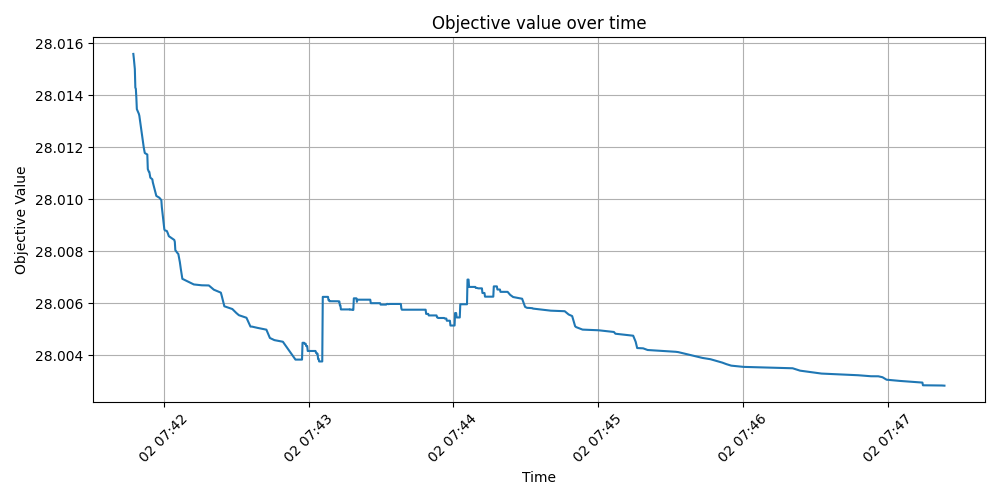
\includegraphics[width=1.0\textwidth]{figures/objective-400-exclusions.png}
	\caption{Figure Caption}
	\label{fig:objective-exclusion-400}
\end{figure}

\subsection{Response to Changes in Knapsack Capacities}
The effects of changes to capacities will be illustrated in the same way as it was with the response to inclusion and below we see the table that shows which inputs that the AbLNS will be affected by.

\begin{table}[H]
	\centering
	\begin{tabular}{|c|c|c|c|c|c|}
	\hline
	                                & \begin{tabular}[c]{@{}c@{}}$\VarMetaTime_1 = 60$\end{tabular} & \begin{tabular}[c]{@{}c@{}}$\VarMetaTime_2 = 120$\end{tabular} & \begin{tabular}[c]{@{}c@{}}$\VarMetaTime_3 = 180$\end{tabular} & \begin{tabular}[c]{@{}c@{}}$\VarMetaTime_4 = 240$\end{tabular} & \begin{tabular}[c]{@{}c@{}}$\VarMetaTime_5 = 300$\end{tabular} \\ \hline
	$\Delta |\SetPeriod|$           & 16                                                            & 16                                                             & 16                                                             & 16                                                             & 16                                                       \\ \hline
	$\Delta |\SetResource|$         & 16                                                            & 16                                                             & 16                                                             & 16                                                             & 16                                                       \\ \hline
	$\Delta |\ParStrategicResource|$& 100                                                           & 200                                                            & 400                                                            & 800                                                            & 1600                                                     \\ \hline
	\end{tabular}
\end{table}

\begin{figure}[H]%% placement specifier
	\centering
	\resizebox{\linewidth}{!}{
		\tikzpicture[gnuplot]
%% generated with GNUPLOT 6.0p1 (Lua 5.2; terminal rev. Jun 2020, script rev. 118)
%% Wed 27 Nov 2024 09:15:11 AM UTC
\path (0.000,0.000) rectangle (16.000,12.000);
\gpcolor{color=gp lt color border}
\gpsetlinetype{gp lt border}
\gpsetdashtype{gp dt solid}
\gpsetlinewidth{1.00}
\draw[gp path] (2.424,2.697)--(2.604,2.697);
\draw[gp path] (15.447,2.697)--(15.267,2.697);
\node[gp node right] at (2.240,2.697) {$1.76\times10^{11}$};
\draw[gp path] (2.424,3.459)--(2.604,3.459);
\draw[gp path] (15.447,3.459)--(15.267,3.459);
\node[gp node right] at (2.240,3.459) {$1.78\times10^{11}$};
\draw[gp path] (2.424,4.220)--(2.604,4.220);
\draw[gp path] (15.447,4.220)--(15.267,4.220);
\node[gp node right] at (2.240,4.220) {$1.8\times10^{11}$};
\draw[gp path] (2.424,4.982)--(2.604,4.982);
\draw[gp path] (15.447,4.982)--(15.267,4.982);
\node[gp node right] at (2.240,4.982) {$1.82\times10^{11}$};
\draw[gp path] (2.424,5.744)--(2.604,5.744);
\draw[gp path] (15.447,5.744)--(15.267,5.744);
\node[gp node right] at (2.240,5.744) {$1.84\times10^{11}$};
\draw[gp path] (2.424,6.505)--(2.604,6.505);
\draw[gp path] (15.447,6.505)--(15.267,6.505);
\node[gp node right] at (2.240,6.505) {$1.86\times10^{11}$};
\draw[gp path] (2.424,7.267)--(2.604,7.267);
\draw[gp path] (15.447,7.267)--(15.267,7.267);
\node[gp node right] at (2.240,7.267) {$1.88\times10^{11}$};
\draw[gp path] (2.424,8.028)--(2.604,8.028);
\draw[gp path] (15.447,8.028)--(15.267,8.028);
\node[gp node right] at (2.240,8.028) {$1.9\times10^{11}$};
\draw[gp path] (2.424,8.790)--(2.604,8.790);
\draw[gp path] (15.447,8.790)--(15.267,8.790);
\node[gp node right] at (2.240,8.790) {$1.92\times10^{11}$};
\draw[gp path] (2.424,9.552)--(2.604,9.552);
\draw[gp path] (15.447,9.552)--(15.267,9.552);
\node[gp node right] at (2.240,9.552) {$1.94\times10^{11}$};
\draw[gp path] (2.424,10.313)--(2.604,10.313);
\draw[gp path] (15.447,10.313)--(15.267,10.313);
\node[gp node right] at (2.240,10.313) {$1.96\times10^{11}$};
\draw[gp path] (2.424,11.075)--(2.604,11.075);
\draw[gp path] (15.447,11.075)--(15.267,11.075);
\node[gp node right] at (2.240,11.075) {$1.98\times10^{11}$};
\draw[gp path] (2.424,2.697)--(2.424,2.517);
\draw[gp path] (2.424,11.075)--(2.424,11.255);
\node[gp node left,rotate=270] at (2.424,2.333) {$1.7327\times10^{9}$};
\draw[gp path] (3.871,2.697)--(3.871,2.517);
\draw[gp path] (3.871,11.075)--(3.871,11.255);
\node[gp node left,rotate=270] at (3.871,2.333) {$1.7327\times10^{9}$};
\draw[gp path] (5.318,2.697)--(5.318,2.517);
\draw[gp path] (5.318,11.075)--(5.318,11.255);
\node[gp node left,rotate=270] at (5.318,2.333) {$1.7327\times10^{9}$};
\draw[gp path] (6.765,2.697)--(6.765,2.517);
\draw[gp path] (6.765,11.075)--(6.765,11.255);
\node[gp node left,rotate=270] at (6.765,2.333) {$1.7327\times10^{9}$};
\draw[gp path] (8.212,2.697)--(8.212,2.517);
\draw[gp path] (8.212,11.075)--(8.212,11.255);
\node[gp node left,rotate=270] at (8.212,2.333) {$1.7327\times10^{9}$};
\draw[gp path] (9.659,2.697)--(9.659,2.517);
\draw[gp path] (9.659,11.075)--(9.659,11.255);
\node[gp node left,rotate=270] at (9.659,2.333) {$1.7327\times10^{9}$};
\draw[gp path] (11.106,2.697)--(11.106,2.517);
\draw[gp path] (11.106,11.075)--(11.106,11.255);
\node[gp node left,rotate=270] at (11.106,2.333) {$1.7327\times10^{9}$};
\draw[gp path] (12.553,2.697)--(12.553,2.517);
\draw[gp path] (12.553,11.075)--(12.553,11.255);
\node[gp node left,rotate=270] at (12.553,2.333) {$1.7327\times10^{9}$};
\draw[gp path] (14.000,2.697)--(14.000,2.517);
\draw[gp path] (14.000,11.075)--(14.000,11.255);
\node[gp node left,rotate=270] at (14.000,2.333) {$1.7327\times10^{9}$};
\draw[gp path] (15.447,2.697)--(15.447,2.517);
\draw[gp path] (15.447,11.075)--(15.447,11.255);
\node[gp node left,rotate=270] at (15.447,2.333) {$1.7327\times10^{9}$};
\draw[gp path] (2.424,11.075)--(2.424,2.697)--(15.447,2.697)--(15.447,11.075)--cycle;
\gpcolor{rgb color={0.580,0.000,0.827}}
\draw[gp path] (3.799,10.388)--(3.799,10.234)--(3.799,10.197)--(3.799,10.174)--(3.799,10.102)%
  --(3.871,10.082)--(3.871,10.068)--(3.871,10.030)--(3.871,9.979)--(3.871,9.963)--(3.871,9.928)%
  --(3.871,9.891)--(3.943,9.872)--(3.943,9.815)--(3.943,9.801)--(3.943,9.794)--(4.016,9.767)%
  --(4.016,9.758)--(4.016,9.745)--(4.016,9.730)--(4.016,9.728)--(4.016,9.722)--(4.016,9.677)%
  --(4.016,9.607)--(4.016,9.606)--(4.088,9.591)--(4.088,9.571)--(4.088,9.524)--(4.160,9.515)%
  --(4.160,9.511)--(4.160,9.486)--(4.160,9.477)--(4.160,9.458)--(4.160,9.454)--(4.160,9.439)%
  --(4.233,9.125)--(4.233,9.022)--(4.233,9.088)--(4.233,8.970)--(4.233,8.854)--(4.305,8.915)%
  --(4.305,8.905)--(4.305,8.861)--(4.377,8.881)--(4.377,8.781)--(4.377,8.831)--(4.450,8.796)%
  --(4.450,8.758)--(4.450,8.832)--(4.450,8.810)--(4.522,8.762)--(4.522,8.723)--(4.522,8.736)%
  --(4.595,8.715)--(4.595,8.698)--(4.667,8.728)--(4.667,8.713)--(4.667,8.658)--(4.667,8.685)%
  --(4.739,8.719)--(4.739,8.701)--(4.739,8.684)--(4.812,8.589)--(4.812,8.622)--(4.812,8.624)%
  --(4.812,8.601)--(4.884,8.653)--(4.884,8.525)--(4.956,8.533)--(4.956,8.606)--(5.029,8.528)%
  --(5.029,8.584)--(5.029,8.591)--(5.101,8.473)--(5.101,8.564)--(5.101,8.552)--(5.101,8.572)%
  --(5.173,8.588)--(5.173,8.615)--(5.246,8.534)--(5.246,8.578)--(5.246,8.586)--(5.318,8.577)%
  --(5.318,8.538)--(5.318,8.482)--(5.318,8.432)--(5.390,8.476)--(5.390,8.475)--(5.390,8.502)%
  --(5.463,8.471)--(5.535,8.479)--(5.535,8.430)--(5.607,8.474)--(5.607,8.375)--(5.607,10.530)%
  --(5.607,10.579)--(5.607,10.529)--(5.680,10.506)--(5.680,10.517)--(5.752,10.471)--(5.752,10.312)%
  --(5.824,10.343)--(5.824,10.417)--(5.824,10.365)--(5.897,10.310)--(5.897,10.307)--(5.897,10.339)%
  --(5.969,10.257)--(5.969,10.335)--(5.969,10.358)--(6.042,10.324)--(6.186,10.276)--(6.186,10.284)%
  --(6.186,10.283)--(6.331,10.281)--(6.476,10.286)--(6.476,10.296)--(6.548,10.265)--(6.548,10.271)%
  --(6.693,10.238)--(6.765,10.266)--(6.837,10.314)--(6.910,10.323)--(6.910,10.302)--(6.982,10.245)%
  --(6.982,10.305)--(6.982,10.275)--(7.054,10.247)--(7.054,10.256)--(7.054,10.243)--(7.054,7.049)%
  --(7.127,7.001)--(7.127,6.919)--(7.127,7.013)--(7.199,6.915)--(7.199,6.858)--(7.199,6.829)%
  --(7.271,6.697)--(7.271,6.666)--(7.271,6.704)--(7.271,6.660)--(7.344,6.698)--(7.344,6.662)%
  --(7.344,6.621)--(7.416,6.616)--(7.416,6.583)--(7.416,6.617)--(7.416,6.608)--(7.489,6.542)%
  --(7.489,6.522)--(7.489,6.443)--(7.561,6.391)--(7.561,6.392)--(7.561,6.287)--(7.633,6.282)%
  --(7.633,6.302)--(7.633,6.305)--(7.706,6.240)--(7.706,6.265)--(7.706,6.282)--(7.778,6.291)%
  --(7.850,6.306)--(7.850,6.199)--(7.850,6.203)--(7.923,6.275)--(7.923,6.284)--(7.995,6.265)%
  --(7.995,6.247)--(8.067,6.220)--(8.067,6.203)--(8.067,6.206)--(8.140,6.182)--(8.140,6.196)%
  --(8.140,6.177)--(8.212,6.151)--(8.212,6.157)--(8.284,6.188)--(8.284,6.142)--(8.357,6.162)%
  --(8.357,6.163)--(8.429,6.168)--(8.429,6.126)--(8.429,6.160)--(8.429,6.167)--(8.501,6.107)%
  --(8.574,3.847)--(8.574,3.843)--(8.574,3.751)--(8.574,3.737)--(8.646,3.752)--(8.646,3.784)%
  --(8.646,3.790)--(8.718,3.777)--(8.718,3.772)--(8.718,3.783)--(8.718,3.768)--(8.791,3.767)%
  --(8.791,3.768)--(8.863,3.652)--(8.863,3.775)--(8.936,3.759)--(8.936,3.698)--(9.008,3.754)%
  --(9.008,3.610)--(9.008,3.604)--(9.008,3.644)--(9.080,3.684)--(9.080,3.628)--(9.153,3.684)%
  --(9.153,3.655)--(9.225,3.668)--(9.225,3.674)--(9.225,3.620)--(9.297,3.655)--(9.297,3.662)%
  --(9.370,3.635)--(9.370,3.608)--(9.442,3.584)--(9.442,3.501)--(9.514,3.487)--(9.587,3.440)%
  --(9.587,3.457)--(9.587,3.485)--(9.587,3.461)--(9.659,3.456)--(9.659,3.416)--(9.731,3.414)%
  --(9.804,3.472)--(9.804,3.445)--(9.876,3.401)--(9.876,3.396)--(9.876,3.437)--(9.948,3.390)%
  --(9.948,3.451)--(9.948,3.423)--(10.021,3.457)--(10.021,3.429)--(10.093,3.464)--(10.093,3.446)%
  --(10.093,3.408)--(10.093,3.471)--(10.165,3.463)--(10.165,3.419)--(10.165,3.481)--(10.238,3.424)%
  --(10.238,3.472)--(10.310,3.371)--(10.310,3.442)--(10.310,3.434)--(10.383,3.398)--(10.383,3.314)%
  --(10.455,3.372)--(10.455,3.274)--(10.455,3.366)--(10.527,3.353)--(10.527,3.386)--(10.600,3.387)%
  --(10.600,3.350)--(10.600,3.336)--(10.600,3.350)--(10.672,3.276)--(10.672,3.293)--(10.744,3.350)%
  --(10.744,3.342)--(10.817,3.316)--(10.817,3.310)--(10.817,3.309)--(10.817,3.347)--(10.889,3.330)%
  --(10.889,3.338)--(10.961,3.326)--(10.961,3.336)--(11.106,3.315)--(11.106,3.343)--(11.106,3.312)%
  --(11.178,3.321)--(11.178,3.337)--(11.178,3.281)--(11.251,3.323)--(11.251,3.328)--(11.251,3.346)%
  --(11.323,3.224)--(11.323,3.345)--(11.395,3.339)--(11.395,3.335)--(11.395,3.344)--(11.468,3.241)%
  --(11.468,3.326)--(11.540,3.288)--(11.540,3.307)--(11.612,3.326)--(11.612,3.277)--(11.612,3.313)%
  --(11.685,3.310)--(11.685,3.311)--(11.685,3.331)--(11.757,3.250)--(11.757,3.313)--(11.757,3.284)%
  --(11.830,3.337)--(11.830,3.335)--(11.902,3.337)--(11.902,3.299)--(11.974,3.283)--(11.974,3.346)%
  --(11.974,3.353)--(12.047,3.337)--(12.047,3.350)--(12.119,3.336)--(12.119,3.345)--(12.191,3.336)%
  --(12.191,3.306)--(12.264,3.310)--(12.264,3.326)--(12.336,3.257)--(12.336,3.322)--(12.408,3.315)%
  --(12.408,3.311)--(12.481,3.310)--(12.481,3.297)--(12.553,3.288)--(12.553,3.296)--(12.625,3.272)%
  --(12.625,3.287)--(12.625,3.262)--(12.698,3.292)--(12.698,3.257)--(12.770,3.276)--(12.770,3.235)%
  --(12.842,3.283)--(12.842,3.245)--(12.915,3.282)--(12.915,3.259)--(12.915,3.234)--(12.987,3.255)%
  --(12.987,3.291)--(13.059,3.292)--(13.059,3.235)--(13.059,3.294)--(13.132,3.276)--(13.132,3.268)%
  --(13.132,3.273)--(13.204,3.268)--(13.277,3.281)--(13.349,3.272)--(13.349,3.279)--(13.421,3.290)%
  --(13.421,3.248)--(13.494,3.279)--(13.566,3.256)--(13.566,3.275)--(13.638,3.278)--(13.638,3.252)%
  --(13.638,3.285)--(13.711,3.219)--(13.711,3.171)--(13.783,3.197)--(13.783,3.281)--(13.855,3.288)%
  --(13.855,3.287)--(13.928,3.246)--(13.928,3.284)--(14.000,3.285)--(14.072,3.269)--(14.072,3.255)%
  --(14.072,3.253)--(14.072,3.209)--(14.145,3.251)--(14.145,3.198)--(14.145,3.242)--(14.217,3.232)%
  --(14.217,3.254)--(14.217,3.250)--(14.289,3.278)--(14.289,3.292)--(14.362,3.285)--(14.362,3.246)%
  --(14.434,3.294)--(14.434,3.302)--(14.434,3.305)--(14.506,3.286)--(14.506,3.276)--(14.579,3.247)%
  --(14.579,3.305)--(14.579,3.233)--(14.651,3.212)--(14.651,3.312)--(14.723,3.287)--(14.723,3.284)%
  --(14.723,3.300)--(14.796,3.216)--(14.796,3.315)--(14.868,3.308)--(14.941,3.301)--(14.941,3.309)%
  --(14.941,3.274)--(15.013,3.320)--(15.013,3.316)--(15.013,3.208)--(15.085,3.329)--(15.158,3.301)%
  --(15.158,3.318)--(15.158,3.264)--(15.230,3.301)--(15.302,3.314)--(15.302,3.285)--(15.302,3.301);
\gpcolor{color=gp lt color border}
\draw[gp path] (2.424,11.075)--(2.424,2.697)--(15.447,2.697)--(15.447,11.075)--cycle;
\node[gp node center,rotate=-270] at (0.292,6.886) {Objective value};
\node[gp node center] at (8.935,0.215) {Absolute time};
\node[gp node center] at (8.935,11.537) {Objective value for Weekly Schedule};
%% coordinates of the plot area
\gpdefrectangularnode{gp plot 1}{\pgfpoint{2.424cm}{2.697cm}}{\pgfpoint{15.447cm}{11.075cm}}
\endtikzpicture
%% gnuplot variables

	}
	\caption{Figure Caption}\label{fig:results:objective-resource-increases}
\end{figure}

Correspondingly we also have the figure below in which the resources are decreasing.

\begin{figure}[H]%% placement specifier
	\centering
	\resizebox{\linewidth}{!}{
		\tikzpicture[gnuplot]
%% generated with GNUPLOT 6.0p1 (Lua 5.2; terminal rev. Jun 2020, script rev. 118)
%% Tue 17 Dec 2024 02:07:05 PM UTC
\path (0.000,0.000) rectangle (16.000,12.000);
\gpcolor{color=gp lt color axes}
\gpsetlinetype{gp lt axes}
\gpsetdashtype{gp dt axes}
\gpsetlinewidth{0.50}
\draw[gp path] (2.424,1.845)--(15.447,1.845);
\gpcolor{color=gp lt color border}
\gpsetlinetype{gp lt border}
\gpsetdashtype{gp dt solid}
\gpsetlinewidth{1.00}
\draw[gp path] (2.424,1.845)--(2.604,1.845);
\draw[gp path] (15.447,1.845)--(15.267,1.845);
\node[gp node right] at (2.240,1.845) {$1.8\times10^{11}$};
\gpcolor{color=gp lt color axes}
\gpsetlinetype{gp lt axes}
\gpsetdashtype{gp dt axes}
\gpsetlinewidth{0.50}
\draw[gp path] (2.424,3.383)--(15.447,3.383);
\gpcolor{color=gp lt color border}
\gpsetlinetype{gp lt border}
\gpsetdashtype{gp dt solid}
\gpsetlinewidth{1.00}
\draw[gp path] (2.424,3.383)--(2.604,3.383);
\draw[gp path] (15.447,3.383)--(15.267,3.383);
\node[gp node right] at (2.240,3.383) {$1.85\times10^{11}$};
\gpcolor{color=gp lt color axes}
\gpsetlinetype{gp lt axes}
\gpsetdashtype{gp dt axes}
\gpsetlinewidth{0.50}
\draw[gp path] (2.424,4.922)--(15.447,4.922);
\gpcolor{color=gp lt color border}
\gpsetlinetype{gp lt border}
\gpsetdashtype{gp dt solid}
\gpsetlinewidth{1.00}
\draw[gp path] (2.424,4.922)--(2.604,4.922);
\draw[gp path] (15.447,4.922)--(15.267,4.922);
\node[gp node right] at (2.240,4.922) {$1.9\times10^{11}$};
\gpcolor{color=gp lt color axes}
\gpsetlinetype{gp lt axes}
\gpsetdashtype{gp dt axes}
\gpsetlinewidth{0.50}
\draw[gp path] (2.424,6.460)--(15.447,6.460);
\gpcolor{color=gp lt color border}
\gpsetlinetype{gp lt border}
\gpsetdashtype{gp dt solid}
\gpsetlinewidth{1.00}
\draw[gp path] (2.424,6.460)--(2.604,6.460);
\draw[gp path] (15.447,6.460)--(15.267,6.460);
\node[gp node right] at (2.240,6.460) {$1.95\times10^{11}$};
\gpcolor{color=gp lt color axes}
\gpsetlinetype{gp lt axes}
\gpsetdashtype{gp dt axes}
\gpsetlinewidth{0.50}
\draw[gp path] (2.424,7.998)--(15.447,7.998);
\gpcolor{color=gp lt color border}
\gpsetlinetype{gp lt border}
\gpsetdashtype{gp dt solid}
\gpsetlinewidth{1.00}
\draw[gp path] (2.424,7.998)--(2.604,7.998);
\draw[gp path] (15.447,7.998)--(15.267,7.998);
\node[gp node right] at (2.240,7.998) {$2\times10^{11}$};
\gpcolor{color=gp lt color axes}
\gpsetlinetype{gp lt axes}
\gpsetdashtype{gp dt axes}
\gpsetlinewidth{0.50}
\draw[gp path] (2.424,9.537)--(15.447,9.537);
\gpcolor{color=gp lt color border}
\gpsetlinetype{gp lt border}
\gpsetdashtype{gp dt solid}
\gpsetlinewidth{1.00}
\draw[gp path] (2.424,9.537)--(2.604,9.537);
\draw[gp path] (15.447,9.537)--(15.267,9.537);
\node[gp node right] at (2.240,9.537) {$2.05\times10^{11}$};
\gpcolor{color=gp lt color axes}
\gpsetlinetype{gp lt axes}
\gpsetdashtype{gp dt axes}
\gpsetlinewidth{0.50}
\draw[gp path] (2.424,11.075)--(15.447,11.075);
\gpcolor{color=gp lt color border}
\gpsetlinetype{gp lt border}
\gpsetdashtype{gp dt solid}
\gpsetlinewidth{1.00}
\draw[gp path] (2.424,11.075)--(2.604,11.075);
\draw[gp path] (15.447,11.075)--(15.267,11.075);
\node[gp node right] at (2.240,11.075) {$2.1\times10^{11}$};
\gpcolor{color=gp lt color axes}
\gpsetlinetype{gp lt axes}
\gpsetdashtype{gp dt axes}
\gpsetlinewidth{0.50}
\draw[gp path] (2.424,1.845)--(2.424,11.075);
\gpcolor{color=gp lt color border}
\gpsetlinetype{gp lt border}
\gpsetdashtype{gp dt solid}
\gpsetlinewidth{1.00}
\draw[gp path] (2.424,1.845)--(2.424,2.025);
\draw[gp path] (2.424,11.075)--(2.424,10.895);
\node[gp node left,rotate=270] at (2.424,1.661) {$0$};
\gpcolor{color=gp lt color axes}
\gpsetlinetype{gp lt axes}
\gpsetdashtype{gp dt axes}
\gpsetlinewidth{0.50}
\draw[gp path] (4.052,1.845)--(4.052,11.075);
\gpcolor{color=gp lt color border}
\gpsetlinetype{gp lt border}
\gpsetdashtype{gp dt solid}
\gpsetlinewidth{1.00}
\draw[gp path] (4.052,1.845)--(4.052,2.025);
\draw[gp path] (4.052,11.075)--(4.052,10.895);
\node[gp node left,rotate=270] at (4.052,1.661) {$50$};
\gpcolor{color=gp lt color axes}
\gpsetlinetype{gp lt axes}
\gpsetdashtype{gp dt axes}
\gpsetlinewidth{0.50}
\draw[gp path] (5.680,1.845)--(5.680,11.075);
\gpcolor{color=gp lt color border}
\gpsetlinetype{gp lt border}
\gpsetdashtype{gp dt solid}
\gpsetlinewidth{1.00}
\draw[gp path] (5.680,1.845)--(5.680,2.025);
\draw[gp path] (5.680,11.075)--(5.680,10.895);
\node[gp node left,rotate=270] at (5.680,1.661) {$100$};
\gpcolor{color=gp lt color axes}
\gpsetlinetype{gp lt axes}
\gpsetdashtype{gp dt axes}
\gpsetlinewidth{0.50}
\draw[gp path] (7.308,1.845)--(7.308,11.075);
\gpcolor{color=gp lt color border}
\gpsetlinetype{gp lt border}
\gpsetdashtype{gp dt solid}
\gpsetlinewidth{1.00}
\draw[gp path] (7.308,1.845)--(7.308,2.025);
\draw[gp path] (7.308,11.075)--(7.308,10.895);
\node[gp node left,rotate=270] at (7.308,1.661) {$150$};
\gpcolor{color=gp lt color axes}
\gpsetlinetype{gp lt axes}
\gpsetdashtype{gp dt axes}
\gpsetlinewidth{0.50}
\draw[gp path] (8.936,1.845)--(8.936,11.075);
\gpcolor{color=gp lt color border}
\gpsetlinetype{gp lt border}
\gpsetdashtype{gp dt solid}
\gpsetlinewidth{1.00}
\draw[gp path] (8.936,1.845)--(8.936,2.025);
\draw[gp path] (8.936,11.075)--(8.936,10.895);
\node[gp node left,rotate=270] at (8.936,1.661) {$200$};
\gpcolor{color=gp lt color axes}
\gpsetlinetype{gp lt axes}
\gpsetdashtype{gp dt axes}
\gpsetlinewidth{0.50}
\draw[gp path] (10.563,1.845)--(10.563,11.075);
\gpcolor{color=gp lt color border}
\gpsetlinetype{gp lt border}
\gpsetdashtype{gp dt solid}
\gpsetlinewidth{1.00}
\draw[gp path] (10.563,1.845)--(10.563,2.025);
\draw[gp path] (10.563,11.075)--(10.563,10.895);
\node[gp node left,rotate=270] at (10.563,1.661) {$250$};
\gpcolor{color=gp lt color axes}
\gpsetlinetype{gp lt axes}
\gpsetdashtype{gp dt axes}
\gpsetlinewidth{0.50}
\draw[gp path] (12.191,1.845)--(12.191,11.075);
\gpcolor{color=gp lt color border}
\gpsetlinetype{gp lt border}
\gpsetdashtype{gp dt solid}
\gpsetlinewidth{1.00}
\draw[gp path] (12.191,1.845)--(12.191,2.025);
\draw[gp path] (12.191,11.075)--(12.191,10.895);
\node[gp node left,rotate=270] at (12.191,1.661) {$300$};
\gpcolor{color=gp lt color axes}
\gpsetlinetype{gp lt axes}
\gpsetdashtype{gp dt axes}
\gpsetlinewidth{0.50}
\draw[gp path] (13.819,1.845)--(13.819,11.075);
\gpcolor{color=gp lt color border}
\gpsetlinetype{gp lt border}
\gpsetdashtype{gp dt solid}
\gpsetlinewidth{1.00}
\draw[gp path] (13.819,1.845)--(13.819,2.025);
\draw[gp path] (13.819,11.075)--(13.819,10.895);
\node[gp node left,rotate=270] at (13.819,1.661) {$350$};
\gpcolor{color=gp lt color axes}
\gpsetlinetype{gp lt axes}
\gpsetdashtype{gp dt axes}
\gpsetlinewidth{0.50}
\draw[gp path] (15.447,1.845)--(15.447,11.075);
\gpcolor{color=gp lt color border}
\gpsetlinetype{gp lt border}
\gpsetdashtype{gp dt solid}
\gpsetlinewidth{1.00}
\draw[gp path] (15.447,1.845)--(15.447,2.025);
\draw[gp path] (15.447,11.075)--(15.447,10.895);
\node[gp node left,rotate=270] at (15.447,1.661) {$400$};
\draw[gp path] (2.424,11.075)--(2.424,1.845)--(15.447,1.845)--(15.447,11.075)--cycle;
\gpcolor{rgb color={0.000,0.000,0.000}}
\gpsetlinewidth{2.00}
\draw[gp path] (2.424,7.213)--(2.424,7.073)--(2.457,7.053)--(2.457,7.025)--(2.457,7.010)%
  --(2.489,6.984)--(2.489,6.971)--(2.489,6.962)--(2.522,6.938)--(2.522,6.921)--(2.522,6.915)%
  --(2.554,6.890)--(2.554,6.848)--(2.554,6.826)--(2.587,6.801)--(2.587,6.788)--(2.587,6.739)%
  --(2.619,6.700)--(2.619,6.698)--(2.619,6.690)--(2.619,6.676)--(2.652,6.651)--(2.652,6.607)%
  --(2.652,6.596)--(2.684,6.595)--(2.684,6.535)--(2.684,6.531)--(2.684,6.496)--(2.717,6.492)%
  --(2.717,6.464)--(2.750,6.426)--(2.750,6.408)--(2.750,6.398)--(2.750,6.386)--(2.750,6.381)%
  --(2.782,6.374)--(2.782,6.364)--(2.782,6.345)--(2.815,6.338)--(2.815,6.333)--(2.847,6.304)%
  --(2.880,6.295)--(2.880,6.294)--(2.912,6.275)--(2.912,6.271)--(2.945,6.262)--(2.945,6.261)%
  --(2.977,6.260)--(2.977,6.254)--(3.010,6.226)--(3.043,6.222)--(3.075,6.214)--(3.108,6.189)%
  --(3.140,6.174)--(3.140,6.158)--(3.173,6.155)--(3.173,6.147)--(3.205,6.145)--(3.205,6.132)%
  --(3.238,6.104)--(3.270,6.097)--(3.336,6.072)--(3.336,6.060)--(3.368,6.051)--(3.368,6.049)%
  --(3.401,6.047)--(3.401,6.046)--(3.401,6.042)--(3.433,6.037)--(3.498,6.028)--(3.498,6.022)%
  --(3.531,6.022)--(3.531,6.018)--(3.564,6.017)--(3.564,6.012)--(3.596,6.008)--(3.596,5.998)%
  --(3.629,5.994)--(3.629,5.989)--(3.661,5.986)--(3.661,5.982)--(3.694,5.982)--(3.759,5.975)%
  --(3.759,5.966)--(3.759,6.043)--(3.759,6.018)--(3.791,6.007)--(3.791,5.978)--(3.791,5.963)%
  --(3.791,5.936)--(3.791,5.935)--(3.791,5.919)--(3.824,5.891)--(3.824,5.868)--(3.824,5.866)%
  --(3.824,5.857)--(3.857,5.840)--(3.857,5.836)--(3.857,5.828)--(3.857,5.817)--(3.889,5.816)%
  --(3.889,5.815)--(3.889,5.808)--(3.889,5.805)--(3.922,5.801)--(3.922,5.795)--(3.922,5.792)%
  --(3.922,5.785)--(3.922,5.782)--(3.954,5.780)--(3.954,5.777)--(3.954,5.774)--(3.987,5.773)%
  --(3.987,5.769)--(3.987,5.764)--(3.987,5.750)--(4.019,5.744)--(4.019,5.742)--(4.019,5.738)%
  --(4.019,5.734)--(4.052,5.741)--(4.052,5.739)--(4.084,5.738)--(4.084,5.736)--(4.084,5.729)%
  --(4.117,5.728)--(4.117,5.727)--(4.117,5.721)--(4.182,5.702)--(4.182,5.710)--(4.182,5.707)%
  --(4.215,5.723)--(4.215,5.716)--(4.247,5.723)--(4.247,5.719)--(4.247,5.716)--(4.247,5.713)%
  --(4.280,5.706)--(4.280,5.717)--(4.312,5.719)--(4.312,5.717)--(4.312,5.716)--(4.377,5.715)%
  --(4.410,5.721)--(4.443,5.720)--(4.443,5.719)--(4.475,5.717)--(4.508,5.716)--(4.508,5.713)%
  --(4.540,5.707)--(4.540,5.702)--(4.573,5.703)--(4.573,5.706)--(4.573,5.704)--(4.605,5.702)%
  --(4.605,5.699)--(4.605,5.697)--(4.638,5.698)--(4.703,5.697)--(4.801,5.696)--(4.801,5.692)%
  --(4.866,5.705)--(4.898,5.703)--(4.898,5.679)--(4.963,5.698)--(5.029,5.696)--(5.061,5.694)%
  --(5.094,5.672)--(5.126,5.672)--(5.159,5.669)--(5.289,5.669)--(5.289,5.667)--(5.354,5.666)%
  --(5.354,5.668)--(5.387,5.666)--(5.419,5.664)--(5.452,3.347)--(5.484,3.339)--(5.484,3.336)%
  --(5.484,3.240)--(5.484,3.233)--(5.517,3.252)--(5.517,3.249)--(5.517,3.243)--(5.517,3.240)%
  --(5.550,3.238)--(5.550,3.225)--(5.550,3.219)--(5.550,3.215)--(5.550,3.213)--(5.582,3.211)%
  --(5.582,3.209)--(5.615,3.137)--(5.615,3.029)--(5.615,3.027)--(5.647,3.070)--(5.647,3.067)%
  --(5.647,3.062)--(5.647,3.061)--(5.680,3.056)--(5.680,3.053)--(5.712,3.050)--(5.712,3.048)%
  --(5.712,3.045)--(5.745,3.043)--(5.745,3.042)--(5.745,3.040)--(5.745,3.038)--(5.777,3.037)%
  --(5.810,3.034)--(5.810,3.033)--(5.810,2.972)--(5.810,2.971)--(5.843,2.970)--(5.843,2.969)%
  --(5.875,2.967)--(5.908,2.965)--(5.908,2.964)--(5.940,2.963)--(6.005,2.961)--(6.038,2.954)%
  --(6.038,2.951)--(6.103,2.948)--(6.103,2.947)--(6.103,2.945)--(6.136,2.945)--(6.168,2.944)%
  --(6.168,2.943)--(6.201,2.939)--(6.331,2.928)--(6.363,2.927)--(6.363,2.923)--(6.396,2.921)%
  --(6.396,2.920)--(6.429,2.919)--(6.461,2.917)--(6.494,2.917)--(6.526,2.916)--(6.559,2.914)%
  --(6.559,2.913)--(6.591,2.912)--(6.624,2.911)--(6.656,2.911)--(6.754,2.910)--(6.852,2.910)%
  --(6.982,2.908)--(7.047,2.905)--(7.112,2.905)--(7.112,2.903)--(7.145,2.903)--(7.177,2.903)%
  --(7.275,2.903)--(7.308,2.902)--(7.405,2.902)--(7.470,2.901)--(7.536,2.900)--(7.568,2.899)%
  --(7.601,2.899)--(7.633,2.897)--(7.666,2.896)--(7.731,2.895)--(7.796,2.894)--(7.829,2.894)%
  --(7.926,2.893)--(8.056,2.891)--(8.122,2.899)--(8.154,2.899)--(8.187,2.899)--(8.187,2.898)%
  --(8.349,2.896)--(8.447,2.896)--(8.480,2.895)--(8.610,2.894)--(8.675,2.894)--(8.740,6.342)%
  --(8.740,6.268)--(8.740,6.200)--(8.740,6.166)--(8.773,6.101)--(8.773,6.057)--(8.773,6.008)%
  --(8.773,5.924)--(8.773,5.888)--(8.773,5.875)--(8.805,5.862)--(8.805,5.861)--(8.805,5.828)%
  --(8.805,5.806)--(8.805,5.777)--(8.838,5.755)--(8.838,5.736)--(8.838,5.725)--(8.838,5.717)%
  --(8.838,5.715)--(8.870,5.712)--(8.870,5.665)--(8.903,5.665)--(8.903,5.664)--(8.903,5.660)%
  --(8.936,5.655)--(8.936,5.653)--(8.936,5.647)--(8.968,5.647)--(8.968,5.644)--(8.968,5.643)%
  --(9.001,5.638)--(9.001,5.630)--(9.098,5.623)--(9.196,5.619)--(9.196,5.617)--(9.229,5.615)%
  --(9.229,5.613)--(9.261,5.609)--(9.261,5.608)--(9.294,5.608)--(9.326,5.607)--(9.359,5.604)%
  --(9.424,5.602)--(9.424,5.600)--(9.456,5.600)--(9.456,5.595)--(9.489,5.591)--(9.489,5.589)%
  --(9.522,5.588)--(9.554,5.573)--(9.587,5.569)--(9.619,5.568)--(9.684,5.568)--(9.684,5.565)%
  --(9.717,5.564)--(9.717,5.562)--(9.749,5.562)--(9.749,5.561)--(9.782,5.560)--(9.815,5.559)%
  --(9.815,5.557)--(9.847,5.556)--(9.880,5.553)--(9.945,5.551)--(10.042,5.550)--(10.075,5.547)%
  --(10.108,5.545)--(10.108,5.544)--(10.173,5.543)--(10.173,5.541)--(10.205,5.541)--(10.335,5.537)%
  --(10.563,5.535)--(10.628,5.532)--(10.661,5.531)--(10.661,5.530)--(10.694,5.528)--(10.726,5.526)%
  --(10.759,5.525)--(10.759,5.520)--(10.856,5.520)--(10.954,5.520)--(11.019,5.517)--(11.215,5.512)%
  --(11.247,5.512)--(11.345,5.509)--(11.605,5.508)--(11.638,5.508)--(11.670,5.507)--(11.735,5.507)%
  --(11.735,5.506)--(11.768,5.505)--(11.768,5.504)--(11.801,5.504)--(11.801,5.503)--(11.931,5.502)%
  --(11.931,5.500)--(11.963,5.500)--(11.996,10.368)--(11.996,10.350)--(12.028,10.291)--(12.028,10.272)%
  --(12.028,10.231)--(12.028,10.225)--(12.061,10.197)--(12.094,10.197)--(12.094,10.189)--(12.094,10.188)%
  --(12.126,10.162)--(12.159,10.161)--(12.224,10.159)--(12.224,10.158)--(12.321,10.133)--(12.321,10.123)%
  --(12.354,10.121)--(12.387,10.099)--(12.387,10.094)--(12.484,10.087)--(12.712,10.085)--(12.842,10.082)%
  --(13.363,10.081)--(13.884,10.081);
\gpcolor{color=gp lt color border}
\gpsetlinewidth{1.00}
\draw[gp path] (2.424,11.075)--(2.424,1.845)--(15.447,1.845)--(15.447,11.075)--cycle;
\node[gp node center,rotate=-270] at (-0.812,6.460) {Objective value};
\node[gp node center] at (8.935,0.215) {Relative time ($\tau$) [S]};
\node[gp node center] at (8.935,11.537) {Objective value for Weekly Schedule};
%% coordinates of the plot area
\gpdefrectangularnode{gp plot 1}{\pgfpoint{2.424cm}{1.845cm}}{\pgfpoint{15.447cm}{11.075cm}}
\endtikzpicture
%% gnuplot variables

	}
	\caption{Figure Caption}\label{fig:results:objective-resource-decreases}
\end{figure}



\subsection{Response to Changes in Item Weights}
The final parameter that will be changed is the work order value $\ParStrategicValue$. This section will be more elaborate as we have to show how that the
work orders are rearranged due to the changes in their value across the different periods.

\begin{table}[H]
	\centering
	\begin{tabular}{|c|c|c|c|c|c|}
	\hline
	             & \begin{tabular}[c]{@{}c@{}}$\VarMetaTime_1 = 60$\end{tabular} & \begin{tabular}[c]{@{}c@{}}$\VarMetaTime_2 = 120$\end{tabular} & \begin{tabular}[c]{@{}c@{}}$\VarMetaTime_3 = 180$\end{tabular} & \begin{tabular}[c]{@{}c@{}}$\VarMetaTime_4 = 240$\end{tabular} & \begin{tabular}[c]{@{}c@{}}$\VarMetaTime_5 = 300$\end{tabular} \\ \hline
	$\Delta |\SetWorkOrder[\VarMetaTime_{n}]{} \triangle \SetWorkOrder[\VarMetaTime_{n-1}]{}              |$         & 20                                                       & 40                                                       & 80                                                       & 160                                                      & 320                                                      \\ \hline
	$\Delta |\SetPeriod[\VarMetaTime_{n}]{} \triangle \SetPeriod[\VarMetaTime_{n-1}]{}                    |$         & 26                                                       & 26                                                       & 26                                                       & 26                                                       & 26                                                       \\ \hline
	\makecell{$\Delta |\ParStrategicValue[\VarMetaTime_{n}]| -$\\ $|\ParStrategicValue[\VarMetaTime_{n - 1}]|$}        & $1 \cdot 10^{5}$                                         & $2 \cdot 10^{5}$                                         & $4 \cdot 10^{5}$                                         & $8 \cdot 10^{5}$                                         & $1.6 \cdot 10^{6}$                                       \\ \hline
	\end{tabular}
\end{table}

\begin{figure}[H]%% placement specifier
	\centering
	\definecolor{gp lt color}{named}{dtu-red}
	\resizebox{\linewidth}{!}{
		\tikzpicture[gnuplot]
%% generated with GNUPLOT 6.0p1 (Lua 5.2; terminal rev. Jun 2020, script rev. 118)
%% Mon 13 Jan 2025 06:26:31 PM UTC
\tikzset{every node/.append style={scale=1.00}}
\path (0.000,0.000) rectangle (16.000,12.000);
\gpcolor{rgb color={0.753,0.753,0.753}}
\gpsetlinetype{gp lt border}
\gpsetdashtype{gp dt solid}
\gpsetlinewidth{2.00}
\draw[gp path] (2.240,1.845)--(13.667,1.845);
\gpcolor{color=gp lt color border}
\gpsetlinewidth{1.00}
\draw[gp path] (2.240,1.845)--(2.420,1.845);
\node[gp node right] at (2.056,2.153) {$9\times10^{10}$};
\gpcolor{rgb color={0.753,0.753,0.753}}
\gpsetlinewidth{2.00}
\draw[gp path] (2.240,2.753)--(13.667,2.753);
\gpcolor{color=gp lt color border}
\gpsetlinewidth{1.00}
\draw[gp path] (2.240,2.753)--(2.420,2.753);
\node[gp node right] at (2.056,3.061) {$1\times10^{11}$};
\gpcolor{rgb color={0.753,0.753,0.753}}
\gpsetlinewidth{2.00}
\draw[gp path] (2.240,3.660)--(13.667,3.660);
\gpcolor{color=gp lt color border}
\gpsetlinewidth{1.00}
\draw[gp path] (2.240,3.660)--(2.420,3.660);
\node[gp node right] at (2.056,3.968) {$1.1\times10^{11}$};
\gpcolor{rgb color={0.753,0.753,0.753}}
\gpsetlinewidth{2.00}
\draw[gp path] (2.240,4.568)--(13.667,4.568);
\gpcolor{color=gp lt color border}
\gpsetlinewidth{1.00}
\draw[gp path] (2.240,4.568)--(2.420,4.568);
\node[gp node right] at (2.056,4.876) {$1.2\times10^{11}$};
\gpcolor{rgb color={0.753,0.753,0.753}}
\gpsetlinewidth{2.00}
\draw[gp path] (2.240,5.475)--(13.667,5.475);
\gpcolor{color=gp lt color border}
\gpsetlinewidth{1.00}
\draw[gp path] (2.240,5.475)--(2.420,5.475);
\node[gp node right] at (2.056,5.783) {$1.3\times10^{11}$};
\gpcolor{rgb color={0.753,0.753,0.753}}
\gpsetlinewidth{2.00}
\draw[gp path] (2.240,6.383)--(13.667,6.383);
\gpcolor{color=gp lt color border}
\gpsetlinewidth{1.00}
\draw[gp path] (2.240,6.383)--(2.420,6.383);
\node[gp node right] at (2.056,6.691) {$1.4\times10^{11}$};
\gpcolor{rgb color={0.753,0.753,0.753}}
\gpsetlinewidth{2.00}
\draw[gp path] (2.240,7.291)--(13.667,7.291);
\gpcolor{color=gp lt color border}
\gpsetlinewidth{1.00}
\draw[gp path] (2.240,7.291)--(2.420,7.291);
\node[gp node right] at (2.056,7.599) {$1.5\times10^{11}$};
\gpcolor{rgb color={0.753,0.753,0.753}}
\gpsetlinewidth{2.00}
\draw[gp path] (2.240,8.198)--(13.667,8.198);
\gpcolor{color=gp lt color border}
\gpsetlinewidth{1.00}
\draw[gp path] (2.240,8.198)--(2.420,8.198);
\node[gp node right] at (2.056,8.506) {$1.6\times10^{11}$};
\gpcolor{rgb color={0.753,0.753,0.753}}
\gpsetlinewidth{2.00}
\draw[gp path] (2.240,9.106)--(13.667,9.106);
\gpcolor{color=gp lt color border}
\gpsetlinewidth{1.00}
\draw[gp path] (2.240,9.106)--(2.420,9.106);
\node[gp node right] at (2.056,9.414) {$1.7\times10^{11}$};
\gpcolor{rgb color={0.753,0.753,0.753}}
\gpsetlinewidth{2.00}
\draw[gp path] (2.240,10.013)--(13.667,10.013);
\gpcolor{color=gp lt color border}
\gpsetlinewidth{1.00}
\draw[gp path] (2.240,10.013)--(2.420,10.013);
\node[gp node right] at (2.056,10.321) {$1.8\times10^{11}$};
\gpcolor{rgb color={0.753,0.753,0.753}}
\gpsetlinewidth{2.00}
\draw[gp path] (2.240,10.921)--(13.667,10.921);
\gpcolor{color=gp lt color border}
\gpsetlinewidth{1.00}
\draw[gp path] (2.240,10.921)--(2.420,10.921);
\node[gp node right] at (2.056,11.229) {$1.9\times10^{11}$};
\gpcolor{rgb color={0.753,0.753,0.753}}
\gpsetlinewidth{2.00}
\draw[gp path] (2.240,1.845)--(2.240,10.921);
\gpcolor{color=gp lt color border}
\gpsetlinewidth{1.00}
\draw[gp path] (2.240,1.845)--(2.240,2.025);
\draw[gp path] (2.240,10.921)--(2.240,10.741);
\node[gp node left,rotate=270] at (2.240,1.661) {$0$};
\gpcolor{rgb color={0.753,0.753,0.753}}
\gpsetlinewidth{2.00}
\draw[gp path] (3.872,1.845)--(3.872,10.921);
\gpcolor{color=gp lt color border}
\gpsetlinewidth{1.00}
\draw[gp path] (3.872,1.845)--(3.872,2.025);
\draw[gp path] (3.872,10.921)--(3.872,10.741);
\node[gp node left,rotate=270] at (3.872,1.661) {$60$};
\gpcolor{rgb color={0.753,0.753,0.753}}
\gpsetlinewidth{2.00}
\draw[gp path] (5.505,1.845)--(5.505,10.921);
\gpcolor{color=gp lt color border}
\gpsetlinewidth{1.00}
\draw[gp path] (5.505,1.845)--(5.505,2.025);
\draw[gp path] (5.505,10.921)--(5.505,10.741);
\node[gp node left,rotate=270] at (5.505,1.661) {$120$};
\gpcolor{rgb color={0.753,0.753,0.753}}
\gpsetlinewidth{2.00}
\draw[gp path] (7.137,1.845)--(7.137,10.921);
\gpcolor{color=gp lt color border}
\gpsetlinewidth{1.00}
\draw[gp path] (7.137,1.845)--(7.137,2.025);
\draw[gp path] (7.137,10.921)--(7.137,10.741);
\node[gp node left,rotate=270] at (7.137,1.661) {$180$};
\gpcolor{rgb color={0.753,0.753,0.753}}
\gpsetlinewidth{2.00}
\draw[gp path] (8.770,1.845)--(8.770,10.921);
\gpcolor{color=gp lt color border}
\gpsetlinewidth{1.00}
\draw[gp path] (8.770,1.845)--(8.770,2.025);
\draw[gp path] (8.770,10.921)--(8.770,10.741);
\node[gp node left,rotate=270] at (8.770,1.661) {$240$};
\gpcolor{rgb color={0.753,0.753,0.753}}
\gpsetlinewidth{2.00}
\draw[gp path] (10.402,1.845)--(10.402,10.921);
\gpcolor{color=gp lt color border}
\gpsetlinewidth{1.00}
\draw[gp path] (10.402,1.845)--(10.402,2.025);
\draw[gp path] (10.402,10.921)--(10.402,10.741);
\node[gp node left,rotate=270] at (10.402,1.661) {$300$};
\gpcolor{rgb color={0.753,0.753,0.753}}
\gpsetlinewidth{2.00}
\draw[gp path] (12.035,1.845)--(12.035,10.921);
\gpcolor{color=gp lt color border}
\gpsetlinewidth{1.00}
\draw[gp path] (12.035,1.845)--(12.035,2.025);
\draw[gp path] (12.035,10.921)--(12.035,10.741);
\node[gp node left,rotate=270] at (12.035,1.661) {$360$};
\gpcolor{rgb color={0.753,0.753,0.753}}
\gpsetlinewidth{2.00}
\draw[gp path] (13.667,1.845)--(13.667,10.921);
\gpcolor{color=gp lt color border}
\gpsetlinewidth{1.00}
\draw[gp path] (13.667,1.845)--(13.667,2.025);
\draw[gp path] (13.667,10.921)--(13.667,10.741);
\node[gp node left,rotate=270] at (13.667,1.661) {$420$};
\draw[gp path] (13.667,1.845)--(13.487,1.845);
\node[gp node left] at (13.851,2.153) {$163000$};
\draw[gp path] (13.667,3.358)--(13.487,3.358);
\node[gp node left] at (13.851,3.666) {$164000$};
\draw[gp path] (13.667,4.870)--(13.487,4.870);
\node[gp node left] at (13.851,5.178) {$165000$};
\draw[gp path] (13.667,6.383)--(13.487,6.383);
\node[gp node left] at (13.851,6.691) {$166000$};
\draw[gp path] (13.667,7.896)--(13.487,7.896);
\node[gp node left] at (13.851,8.204) {$167000$};
\draw[gp path] (13.667,9.408)--(13.487,9.408);
\node[gp node left] at (13.851,9.716) {$168000$};
\draw[gp path] (13.667,10.921)--(13.487,10.921);
\node[gp node left] at (13.851,11.229) {$169000$};
\draw[gp path] (2.240,10.921)--(2.240,1.845)--(13.667,1.845)--(13.667,10.921)--cycle;
\draw[gp path] (1.517,11.820)--(1.517,12.590)--(14.389,12.590)--(14.389,11.820)--cycle;
\node[gp node right] at (6.669,12.205) {Strategic Urgency};
\gpcolor{rgb color={0.000,0.000,0.000}}
\gpsetlinewidth{2.50}
\draw[gp path] (6.853,12.205)--(7.769,12.205);
\draw[gp path] (2.240,2.378)--(2.240,2.376)--(2.240,2.384)--(2.267,2.385)--(2.267,2.392)%
  --(2.267,2.395)--(2.267,2.396)--(2.267,2.414)--(2.294,2.415)--(2.294,2.418)--(2.294,2.417)%
  --(2.294,2.419)--(2.294,2.423)--(2.322,2.428)--(2.322,2.432)--(2.322,2.436)--(2.322,2.437)%
  --(2.322,2.438)--(2.349,2.439)--(2.349,2.443)--(2.349,2.445)--(2.349,2.444)--(2.349,2.445)%
  --(2.376,2.446)--(2.376,2.447)--(2.376,2.449)--(2.376,2.452)--(2.403,2.459)--(2.403,2.460)%
  --(2.403,2.462)--(2.403,2.465)--(2.403,2.468)--(2.403,2.471)--(2.430,2.471)--(2.430,2.487)%
  --(2.430,2.481)--(2.430,2.485)--(2.430,2.487)--(2.430,2.494)--(2.430,2.493)--(2.458,2.497)%
  --(2.458,2.498)--(2.458,2.505)--(2.458,2.510)--(2.458,2.515)--(2.458,2.522)--(2.485,2.519)%
  --(2.485,2.532)--(2.485,2.531)--(2.485,2.527)--(2.512,2.526)--(2.512,2.524)--(2.512,2.528)%
  --(2.512,2.524)--(2.512,2.526)--(2.539,2.526)--(2.539,2.528)--(2.566,2.533)--(2.566,2.535)%
  --(2.566,2.549)--(2.566,2.546)--(2.594,2.545)--(2.594,2.547)--(2.594,2.546)--(2.594,2.544)%
  --(2.594,2.541)--(2.621,2.539)--(2.621,2.538)--(2.621,2.540)--(2.648,2.540)--(2.648,2.539)%
  --(2.648,2.537)--(2.675,2.536)--(2.675,2.537)--(2.675,2.539)--(2.675,2.553)--(2.703,2.552)%
  --(2.703,2.556)--(2.703,2.555)--(2.730,2.554)--(2.730,2.552)--(2.730,2.551)--(2.757,2.550)%
  --(2.784,2.549)--(2.784,2.545)--(2.811,2.551)--(2.839,2.548)--(2.839,2.549)--(2.839,2.545)%
  --(2.866,2.556)--(2.866,2.554)--(2.893,2.553)--(2.893,2.555)--(2.920,2.559)--(2.920,2.561)%
  --(2.920,2.559)--(2.920,2.555)--(2.947,2.553)--(2.947,2.552)--(2.947,2.548)--(2.947,2.549)%
  --(2.975,2.548)--(2.975,2.546)--(3.002,2.542)--(3.002,2.543)--(3.002,2.541)--(3.056,2.536)%
  --(3.083,2.534)--(3.111,2.535)--(3.138,2.535)--(3.192,2.534)--(3.219,2.537)--(3.247,2.534)%
  --(3.247,2.532)--(3.274,2.530)--(3.301,2.529)--(3.301,2.527)--(3.301,2.529)--(3.301,2.530)%
  --(3.328,2.527)--(3.383,2.526)--(3.383,2.525)--(3.410,2.534)--(3.464,2.532)--(3.492,2.523)%
  --(3.519,2.523)--(3.519,2.522)--(3.519,2.521)--(3.573,2.519)--(3.573,2.518)--(3.628,2.517)%
  --(3.655,2.516)--(3.682,2.514)--(3.709,2.513)--(3.736,2.513)--(3.818,2.512)--(3.845,2.515)%
  --(3.845,2.513)--(3.872,2.512)--(3.900,2.511)--(3.954,3.525)--(3.954,3.521)--(3.954,3.517)%
  --(3.954,3.515)--(3.981,3.515)--(3.981,3.507)--(3.981,3.504)--(4.008,3.501)--(4.036,3.501)%
  --(4.036,3.497)--(4.036,3.507)--(4.063,3.507)--(4.063,3.509)--(4.090,3.508)--(4.090,3.506)%
  --(4.090,3.496)--(4.117,3.489)--(4.117,3.487)--(4.117,3.486)--(4.145,3.484)--(4.145,3.482)%
  --(4.172,3.480)--(4.172,3.482)--(4.172,3.471)--(4.199,3.472)--(4.199,3.470)--(4.199,3.475)%
  --(4.199,3.474)--(4.226,3.473)--(4.226,3.475)--(4.226,3.476)--(4.226,3.477)--(4.253,3.476)%
  --(4.253,3.471)--(4.253,3.470)--(4.253,3.471)--(4.281,3.472)--(4.308,3.465)--(4.335,3.464)%
  --(4.362,3.464)--(4.362,3.466)--(4.362,3.467)--(4.389,3.464)--(4.417,3.458)--(4.417,3.460)%
  --(4.444,3.462)--(4.444,3.463)--(4.444,3.461)--(4.498,3.462)--(4.525,3.461)--(4.553,3.460)%
  --(4.553,3.458)--(4.580,3.459)--(4.607,3.459)--(4.607,3.460)--(4.634,3.458)--(4.634,3.454)%
  --(4.661,3.452)--(4.689,3.454)--(4.689,3.452)--(4.716,3.449)--(4.716,3.450)--(4.852,3.449)%
  --(4.906,3.450)--(4.906,3.446)--(4.934,3.446)--(4.988,3.445)--(5.015,3.444)--(5.124,3.440)%
  --(5.151,3.439)--(5.151,3.438)--(5.178,3.436)--(5.233,3.435)--(5.287,3.437)--(5.342,3.437)%
  --(5.369,3.434)--(5.396,3.433)--(5.423,3.432)--(5.478,3.432)--(5.532,3.431)--(5.586,4.769)%
  --(5.586,4.767)--(5.586,4.760)--(5.586,4.758)--(5.614,4.755)--(5.614,4.752)--(5.614,4.751)%
  --(5.614,4.712)--(5.614,4.706)--(5.641,4.708)--(5.641,4.711)--(5.641,4.712)--(5.641,4.703)%
  --(5.668,4.697)--(5.668,4.696)--(5.668,4.699)--(5.668,4.687)--(5.668,4.684)--(5.695,4.683)%
  --(5.695,4.693)--(5.695,4.694)--(5.723,4.693)--(5.723,4.690)--(5.723,4.696)--(5.750,4.697)%
  --(5.750,4.707)--(5.777,4.706)--(5.777,4.699)--(5.804,4.704)--(5.804,4.701)--(5.804,4.699)%
  --(5.831,4.700)--(5.831,4.702)--(5.831,4.699)--(5.859,4.699)--(5.859,4.691)--(5.859,4.693)%
  --(5.859,4.692)--(5.886,4.674)--(5.913,4.674)--(5.913,4.678)--(5.913,4.681)--(5.940,4.687)%
  --(5.940,4.689)--(5.967,4.685)--(5.967,4.684)--(5.995,4.683)--(6.022,4.680)--(6.049,4.680)%
  --(6.049,4.679)--(6.076,4.678)--(6.076,4.677)--(6.103,4.675)--(6.131,4.673)--(6.212,4.670)%
  --(6.212,4.668)--(6.212,4.667)--(6.239,4.663)--(6.267,4.659)--(6.321,4.662)--(6.321,4.664)%
  --(6.348,4.665)--(6.348,4.666)--(6.348,4.665)--(6.375,4.666)--(6.375,4.665)--(6.403,4.663)%
  --(6.430,4.660)--(6.430,4.657)--(6.457,4.656)--(6.484,4.654)--(6.484,4.653)--(6.512,4.656)%
  --(6.512,4.655)--(6.512,4.652)--(6.593,4.651)--(6.648,4.650)--(6.675,4.650)--(6.675,4.649)%
  --(6.784,4.649)--(6.811,4.647)--(6.865,4.643)--(6.892,4.641)--(6.947,4.642)--(7.083,4.640)%
  --(7.110,4.639)--(7.137,4.638)--(7.219,4.636)--(7.219,5.523)--(7.219,5.515)--(7.219,5.513)%
  --(7.246,5.513)--(7.246,5.515)--(7.246,5.511)--(7.273,5.510)--(7.273,5.508)--(7.273,5.504)%
  --(7.273,5.508)--(7.301,5.510)--(7.301,5.508)--(7.328,5.507)--(7.328,5.491)--(7.328,5.490)%
  --(7.355,5.482)--(7.355,5.487)--(7.382,5.487)--(7.382,5.489)--(7.382,5.486)--(7.409,5.483)%
  --(7.409,5.489)--(7.409,5.487)--(7.437,5.473)--(7.464,5.472)--(7.464,5.469)--(7.464,5.468)%
  --(7.491,5.467)--(7.491,5.465)--(7.491,5.460)--(7.518,5.451)--(7.518,5.450)--(7.545,5.459)%
  --(7.545,5.458)--(7.545,5.456)--(7.573,5.458)--(7.573,5.452)--(7.600,5.450)--(7.627,5.450)%
  --(7.654,5.448)--(7.681,5.446)--(7.681,5.447)--(7.681,5.446)--(7.709,5.445)--(7.763,5.443)%
  --(7.790,5.442)--(7.872,5.439)--(7.899,5.442)--(7.899,5.443)--(7.926,5.436)--(8.008,5.439)%
  --(8.008,5.438)--(8.008,5.445)--(8.035,5.434)--(8.090,5.431)--(8.117,5.432)--(8.144,5.430)%
  --(8.226,5.429)--(8.253,5.430)--(8.307,5.427)--(8.362,5.427)--(8.389,5.426)--(8.389,5.424)%
  --(8.389,5.421)--(8.389,5.417)--(8.443,5.416)--(8.443,5.422)--(8.470,5.421)--(8.525,5.421)%
  --(8.552,5.422)--(8.579,5.421)--(8.606,5.427)--(8.606,5.426)--(8.661,5.423)--(8.661,5.421)%
  --(8.770,5.420)--(8.824,5.419)--(8.851,5.419)--(8.879,8.433)--(8.879,8.429)--(8.879,8.425)%
  --(8.879,8.422)--(8.879,8.424)--(8.879,8.423)--(8.906,8.419)--(8.906,8.416)--(8.906,8.417)%
  --(8.906,8.425)--(8.933,8.429)--(8.933,8.425)--(8.933,8.421)--(8.933,8.415)--(8.933,8.411)%
  --(8.960,8.403)--(8.960,8.395)--(8.987,8.394)--(8.987,8.395)--(8.987,8.376)--(8.987,8.388)%
  --(9.015,8.379)--(9.015,8.378)--(9.015,8.372)--(9.042,8.369)--(9.042,8.367)--(9.069,8.364)%
  --(9.069,8.365)--(9.096,8.362)--(9.123,8.360)--(9.178,8.359)--(9.205,8.359)--(9.205,8.361)%
  --(9.232,8.359)--(9.259,8.357)--(9.259,8.354)--(9.314,8.362)--(9.314,8.360)--(9.314,8.359)%
  --(9.341,8.354)--(9.341,8.353)--(9.341,8.354)--(9.368,8.354)--(9.395,8.358)--(9.395,8.359)%
  --(9.423,8.358)--(9.450,8.363)--(9.450,8.364)--(9.477,8.363)--(9.613,8.361)--(9.613,8.362)%
  --(9.722,8.358)--(9.858,8.356)--(9.912,8.352)--(9.912,8.351)--(9.994,8.351)--(9.994,8.349)%
  --(10.021,8.347)--(10.021,8.339)--(10.048,8.336)--(10.130,8.334)--(10.157,8.334)--(10.266,8.340)%
  --(10.266,8.337)--(10.348,8.336)--(10.429,8.342)--(10.484,8.340)--(10.511,10.545)--(10.511,10.536)%
  --(10.511,10.534)--(10.538,10.534)--(10.538,10.531)--(10.538,10.525)--(10.565,10.532)--(10.565,10.528)%
  --(10.593,10.528)--(10.593,10.523)--(10.593,10.520)--(10.620,10.517)--(10.620,10.518)--(10.620,10.513)%
  --(10.647,10.511)--(10.647,10.510)--(10.647,10.513)--(10.674,10.511)--(10.674,10.516)--(10.701,10.516)%
  --(10.701,10.513)--(10.756,10.512)--(10.783,10.516)--(10.783,10.513)--(10.783,10.511)--(10.837,10.507)%
  --(10.837,10.504)--(10.865,10.503)--(10.892,10.504)--(10.919,10.504)--(10.919,10.506)--(10.919,10.504)%
  --(10.919,10.494)--(10.946,10.490)--(10.973,10.488)--(11.055,10.482)--(11.082,10.482)--(11.110,10.481)%
  --(11.246,10.482)--(11.300,10.480)--(11.327,10.478)--(11.354,10.476)--(11.409,10.475)--(11.436,10.475)%
  --(11.463,10.470)--(11.490,10.474)--(11.518,10.474)--(11.545,10.469)--(11.572,10.467)--(11.572,10.469)%
  --(11.626,10.469)--(11.681,10.470)--(11.708,10.470)--(11.844,10.470)--(11.844,10.469)--(11.844,10.467)%
  --(11.926,10.466)--(11.980,10.469)--(12.007,10.468)--(12.062,10.463);
\gpcolor{color=gp lt color border}
\node[gp node right] at (13.105,12.205) {Strategic Resource Penalty};
\gpcolor{rgb color={0.184,0.243,0.918}}
\draw[gp path] (13.289,12.205)--(14.205,12.205);
\draw[gp path] (2.240,10.278)--(2.240,10.122)--(2.240,9.938)--(2.267,9.726)--(2.267,9.653)%
  --(2.267,9.495)--(2.267,9.287)--(2.267,9.154)--(2.294,9.059)--(2.294,8.893)--(2.294,8.717)%
  --(2.294,8.631)--(2.294,8.313)--(2.322,8.292)--(2.322,8.192)--(2.322,8.056)--(2.322,7.933)%
  --(2.322,7.847)--(2.349,7.809)--(2.349,7.643)--(2.349,7.589)--(2.349,7.555)--(2.349,7.454)%
  --(2.376,7.452)--(2.376,7.428)--(2.376,7.244)--(2.376,7.153)--(2.403,7.027)--(2.403,6.974)%
  --(2.403,6.835)--(2.403,6.676)--(2.403,6.611)--(2.403,6.483)--(2.430,6.451)--(2.430,6.359)%
  --(2.430,6.338)--(2.430,6.324)--(2.430,6.280)--(2.430,6.227)--(2.430,6.185)--(2.458,6.162)%
  --(2.458,6.146)--(2.458,6.102)--(2.458,6.058)--(2.458,5.975)--(2.458,5.929)--(2.458,5.885)%
  --(2.485,5.813)--(2.485,5.698)--(2.485,5.680)--(2.485,5.668)--(2.512,5.616)--(2.512,5.605)%
  --(2.512,5.542)--(2.512,5.491)--(2.512,5.451)--(2.539,5.427)--(2.539,5.406)--(2.539,5.341)%
  --(2.566,5.321)--(2.566,5.291)--(2.566,5.289)--(2.566,5.274)--(2.594,5.273)--(2.594,5.217)%
  --(2.594,5.202)--(2.594,5.156)--(2.594,5.137)--(2.621,5.085)--(2.621,5.079)--(2.621,5.059)%
  --(2.648,5.059)--(2.648,5.020)--(2.648,4.993)--(2.675,4.981)--(2.675,4.963)--(2.675,4.946)%
  --(2.675,4.928)--(2.675,4.693)--(2.703,4.678)--(2.703,4.394)--(2.730,4.364)--(2.730,4.355)%
  --(2.757,4.341)--(2.784,4.338)--(2.784,4.333)--(2.811,4.320)--(2.839,4.320)--(2.839,4.296)%
  --(2.866,4.285)--(2.866,4.279)--(2.893,4.279)--(2.893,4.268)--(2.920,4.262)--(2.920,3.948)%
  --(2.920,3.905)--(2.920,3.904)--(2.947,3.904)--(2.947,3.899)--(2.947,3.895)--(2.975,3.895)%
  --(2.975,3.893)--(3.002,3.867)--(3.002,3.864)--(3.002,3.825)--(3.056,3.810)--(3.083,3.810)%
  --(3.083,3.786)--(3.111,3.778)--(3.138,3.768)--(3.192,3.768)--(3.219,3.766)--(3.247,3.765)%
  --(3.274,3.765)--(3.301,3.765)--(3.301,3.749)--(3.301,3.742)--(3.328,3.742)--(3.383,3.742)%
  --(3.410,3.719)--(3.410,3.710)--(3.464,3.710)--(3.492,3.710)--(3.519,3.710)--(3.573,3.698)%
  --(3.628,3.698)--(3.655,3.698)--(3.682,3.698)--(3.709,3.698)--(3.736,3.697)--(3.818,3.697)%
  --(3.845,3.672)--(3.872,3.672)--(3.900,3.662)--(3.954,4.766)--(3.954,4.721)--(3.954,4.569)%
  --(3.954,4.565)--(3.981,4.562)--(3.981,4.533)--(3.981,4.515)--(4.008,4.479)--(4.036,4.479)%
  --(4.036,4.473)--(4.036,4.459)--(4.036,4.451)--(4.063,4.445)--(4.063,4.441)--(4.090,4.429)%
  --(4.090,4.338)--(4.117,4.314)--(4.117,4.306)--(4.117,4.276)--(4.145,4.253)--(4.145,4.227)%
  --(4.172,4.220)--(4.172,4.194)--(4.172,4.165)--(4.199,4.147)--(4.199,4.137)--(4.199,4.123)%
  --(4.226,4.111)--(4.226,4.076)--(4.226,4.067)--(4.226,4.064)--(4.253,3.914)--(4.253,3.902)%
  --(4.253,3.896)--(4.281,3.892)--(4.308,3.892)--(4.335,3.892)--(4.362,3.892)--(4.362,3.884)%
  --(4.362,3.849)--(4.389,3.849)--(4.417,3.825)--(4.417,3.777)--(4.444,3.771)--(4.444,3.734)%
  --(4.498,3.719)--(4.525,3.695)--(4.553,3.677)--(4.580,3.672)--(4.607,3.669)--(4.607,3.668)%
  --(4.634,3.666)--(4.661,3.666)--(4.689,3.662)--(4.716,3.644)--(4.716,3.641)--(4.852,3.628)%
  --(4.906,3.619)--(4.906,3.603)--(4.934,3.603)--(4.988,3.603)--(5.015,3.574)--(5.124,3.574)%
  --(5.151,3.571)--(5.178,3.568)--(5.233,3.568)--(5.287,3.320)--(5.342,3.320)--(5.369,3.320)%
  --(5.396,3.296)--(5.423,3.296)--(5.478,3.281)--(5.532,3.281)--(5.586,4.780)--(5.586,4.774)%
  --(5.586,4.698)--(5.614,4.649)--(5.614,4.612)--(5.614,4.547)--(5.614,4.197)--(5.614,4.122)%
  --(5.641,4.109)--(5.641,4.011)--(5.641,4.004)--(5.641,3.943)--(5.668,3.937)--(5.668,3.884)%
  --(5.668,3.867)--(5.668,3.737)--(5.695,3.737)--(5.695,3.700)--(5.695,3.580)--(5.723,3.580)%
  --(5.723,3.563)--(5.723,3.495)--(5.750,3.448)--(5.750,3.442)--(5.777,3.432)--(5.777,3.371)%
  --(5.804,3.370)--(5.804,3.359)--(5.831,3.358)--(5.831,3.294)--(5.859,3.290)--(5.859,3.282)%
  --(5.859,3.252)--(5.886,3.105)--(5.913,3.105)--(5.913,3.096)--(5.913,3.091)--(5.940,3.084)%
  --(5.940,3.075)--(5.967,3.014)--(5.995,3.004)--(6.022,3.004)--(6.049,3.004)--(6.076,3.004)%
  --(6.076,2.961)--(6.076,2.937)--(6.103,2.937)--(6.131,2.937)--(6.212,2.937)--(6.212,2.934)%
  --(6.239,2.934)--(6.267,2.934)--(6.321,2.928)--(6.321,2.916)--(6.321,2.913)--(6.348,2.905)%
  --(6.348,2.899)--(6.375,2.890)--(6.375,2.878)--(6.403,2.878)--(6.430,2.878)--(6.457,2.875)%
  --(6.484,2.875)--(6.512,2.848)--(6.593,2.848)--(6.648,2.848)--(6.675,2.834)--(6.784,2.827)%
  --(6.811,2.827)--(6.865,2.827)--(6.892,2.821)--(6.947,2.803)--(7.083,2.790)--(7.110,2.790)%
  --(7.137,2.790)--(7.219,2.790)--(7.219,4.165)--(7.219,4.093)--(7.219,4.081)--(7.246,4.066)%
  --(7.246,4.034)--(7.246,4.005)--(7.246,3.889)--(7.273,3.881)--(7.273,3.840)--(7.273,3.819)%
  --(7.273,3.721)--(7.301,3.719)--(7.301,3.713)--(7.328,3.710)--(7.328,3.491)--(7.355,3.418)%
  --(7.355,3.409)--(7.382,3.395)--(7.382,3.386)--(7.409,3.386)--(7.409,3.373)--(7.409,3.344)%
  --(7.409,3.336)--(7.409,3.329)--(7.437,3.184)--(7.464,3.184)--(7.464,3.160)--(7.464,3.153)%
  --(7.491,3.135)--(7.491,3.117)--(7.491,3.111)--(7.518,3.094)--(7.545,3.091)--(7.545,3.069)%
  --(7.573,3.020)--(7.573,3.008)--(7.600,3.005)--(7.627,3.005)--(7.654,2.998)--(7.681,2.998)%
  --(7.681,2.989)--(7.709,2.952)--(7.763,2.952)--(7.790,2.952)--(7.872,2.952)--(7.872,2.936)%
  --(7.872,2.913)--(7.899,2.910)--(7.899,2.907)--(7.926,2.893)--(8.008,2.881)--(8.008,2.875)%
  --(8.035,2.875)--(8.090,2.875)--(8.117,2.828)--(8.144,2.812)--(8.226,2.812)--(8.253,2.796)%
  --(8.307,2.781)--(8.362,2.781)--(8.389,2.780)--(8.389,2.778)--(8.389,2.745)--(8.443,2.745)%
  --(8.443,2.509)--(8.470,2.506)--(8.525,2.505)--(8.552,2.503)--(8.579,2.503)--(8.606,2.480)%
  --(8.661,2.477)--(8.770,2.474)--(8.824,2.456)--(8.851,2.456)--(8.879,3.937)--(8.879,3.932)%
  --(8.879,3.881)--(8.879,3.852)--(8.879,3.724)--(8.879,3.701)--(8.906,3.701)--(8.906,3.659)%
  --(8.906,3.650)--(8.906,3.641)--(8.933,3.477)--(8.933,3.464)--(8.933,3.324)--(8.933,3.261)%
  --(8.933,3.209)--(8.960,3.184)--(8.960,3.107)--(8.987,2.958)--(8.987,2.940)--(8.987,2.922)%
  --(8.987,2.754)--(8.987,2.731)--(9.015,2.719)--(9.015,2.680)--(9.042,2.591)--(9.069,2.591)%
  --(9.069,2.585)--(9.096,2.582)--(9.123,2.554)--(9.178,2.536)--(9.205,2.518)--(9.205,2.517)%
  --(9.232,2.511)--(9.259,2.511)--(9.314,2.505)--(9.314,2.501)--(9.341,2.470)--(9.341,2.452)%
  --(9.368,2.452)--(9.395,2.438)--(9.395,2.432)--(9.423,2.432)--(9.450,2.429)--(9.450,2.411)%
  --(9.477,2.411)--(9.613,2.411)--(9.613,2.387)--(9.722,2.387)--(9.858,2.387)--(9.912,2.387)%
  --(9.994,2.382)--(9.994,2.355)--(10.021,2.355)--(10.048,2.355)--(10.130,2.353)--(10.157,2.346)%
  --(10.266,2.335)--(10.266,2.334)--(10.348,2.334)--(10.429,2.325)--(10.484,2.318)--(10.511,3.365)%
  --(10.511,3.234)--(10.511,3.209)--(10.538,3.203)--(10.538,3.182)--(10.538,3.169)--(10.565,3.167)%
  --(10.565,3.155)--(10.565,3.113)--(10.593,3.110)--(10.593,3.049)--(10.593,2.973)--(10.620,2.955)%
  --(10.620,2.924)--(10.620,2.600)--(10.647,2.585)--(10.647,2.553)--(10.647,2.547)--(10.647,2.545)%
  --(10.674,2.545)--(10.674,2.529)--(10.701,2.529)--(10.701,2.517)--(10.701,2.515)--(10.756,2.515)%
  --(10.783,2.492)--(10.783,2.456)--(10.837,2.397)--(10.837,2.385)--(10.865,2.380)--(10.892,2.371)%
  --(10.919,2.362)--(10.919,2.340)--(10.919,2.223)--(10.946,2.199)--(10.973,2.199)--(11.055,2.196)%
  --(11.082,2.196)--(11.110,2.193)--(11.246,2.170)--(11.300,2.149)--(11.327,2.141)--(11.354,2.129)%
  --(11.409,2.120)--(11.436,2.111)--(11.463,2.095)--(11.490,2.089)--(11.518,2.089)--(11.545,2.082)%
  --(11.572,2.082)--(11.572,2.073)--(11.626,2.061)--(11.681,2.049)--(11.708,2.049)--(11.844,2.042)%
  --(11.844,2.034)--(11.844,2.023)--(11.926,2.023)--(11.980,2.016)--(12.007,2.016)--(12.062,1.990);
\gpcolor{color=gp lt color border}
\gpsetlinewidth{1.00}
\draw[gp path] (2.240,10.921)--(2.240,1.845)--(13.667,1.845)--(13.667,10.921)--cycle;
\node[gp node center,rotate=-270] at (-0.628,6.383) {Strategic Urgency [Weighted Tardiness]};
\node[gp node center,rotate=-270] at (16.213,6.383) {Strategic Resource Penalty [Hours]};
\node[gp node center] at (7.953,0.215) {Relative time ($\tau$) [Seconds]};
%% coordinates of the plot area
\gpdefrectangularnode{gp plot 1}{\pgfpoint{2.240cm}{1.845cm}}{\pgfpoint{13.667cm}{10.921cm}}
\endtikzpicture
%% gnuplot variables

	}
	\caption{Figure Caption}\label{fig:results:objective-weight-change}
\end{figure}
